% !TeX program = pdfLaTeX
% Proyecto autocontenido para Overleaf. Compilar main.tex con pdfLaTeX.
% Los comentarios REUTILIZADO identifican la procedencia del texto conservado.
\documentclass[11pt,letterpaper]{article}
\usepackage[utf8]{inputenc}
\usepackage[T1]{fontenc}
\usepackage{lmodern}
\IfFileExists{spanish.ldf}{\usepackage[spanish,es-tabla]{babel}}{%
  \usepackage{babel}\babelprovide[main,import]{spanish}%
  \addto\captionsspanish{\renewcommand{\tablename}{Tabla}\renewcommand{\figurename}{Figura}}}
\usepackage[margin=2.2cm]{geometry}
\usepackage{microtype,booktabs,array,xcolor,graphicx,eso-pic,titlesec,caption,amsmath,float}
\usepackage[authoryear,round,sort]{natbib}
\usepackage[colorlinks=true,linkcolor=black,citecolor=black,urlcolor=blue!50!black]{hyperref}
\setlength{\parskip}{3pt}
\setlength{\parindent}{0pt}
\titlespacing*{\section}{0pt}{9pt}{4pt}
\titlespacing*{\subsection}{0pt}{6pt}{2pt}
\titleformat{\section}{\large\bfseries}{\thesection.}{0.5em}{}
\titleformat{\subsection}{\normalsize\bfseries}{\thesubsection}{0.5em}{}
\captionsetup{font=small,skip=4pt,labelsep=period}
\setlength{\textfloatsep}{9pt}
\setlength{\intextsep}{6pt}
\renewcommand{\topfraction}{0.9}
\renewcommand{\bottomfraction}{0.9}
\renewcommand{\textfraction}{0.07}
\renewcommand{\floatpagefraction}{0.85}
\setcounter{totalnumber}{5}
\newcolumntype{P}[1]{>{\raggedright\arraybackslash}p{#1}}
\newcommand{\Othree}{O$_3$}
\newcommand{\NOx}{NO$_x$}
\newcommand{\ppb}{\,ppb}
\newcommand{\nota}[1]{{\footnotesize #1\par}}
\newcommand{\figura}[4]{\begin{figure}[H]\centering\includegraphics[width=#2\textwidth]{img/#1}\caption{#3}\label{#4}\end{figure}}
\renewcommand{\bibsection}{\section*{Referencias}}
\setlength{\bibsep}{7pt}
\renewcommand{\bibfont}{\small}
\hypersetup{pdftitle={Datos en el Aire. Informe final SIMA},pdfauthor={Equipo 3}}
\newenvironment{cambio}{}{}
\begin{document}
\ifdefined\decimalpoint\decimalpoint\fi
\hypersetup{pageanchor=false}

% REUTILIZADO: portada de los entregables 1 y 2; se actualizan etapa y fecha.
\begin{titlepage}
\AddToShipoutPictureBG*{%
  \AtPageLowerLeft{%
    \put(-364,\LenToUnit{0.5\paperheight}){%
      \raisebox{-0.5\height}{
\includegraphics[width=707pt]{img/tec_watermark.png}}}}}
\centering
\vspace*{1.2cm}

\includegraphics[width=6.6cm]{img/tec_logo.png}\par
\vspace{3.6cm}
{\Large\bfseries Datos en el Aire: Análisis Multivariado de la Calidad del Aire en la Zona Metropolitana de Monterrey\par}
\vspace{0.4cm}
{\large Etapa 4: Informe final del Reto\par}
\vspace{0.3cm}
{\normalsize Relaciones entre precursores, meteorología y ozono; clasificación de días con excedencia en SIMA, 2021--2025\par}
\vspace{1.6cm}
Miembros\\Equipo 3\\[6pt]
Ricardo Ballesteros Amavizca \hfill A01255358\\
Landon Mauricio Treviño Ortiz \hfill A01199312\\
Josué Olvera Zozaya \hfill A00842044\\[6pt]
Repositorio: \url{https://github.com/Ricardo-B04/sima-monitoreo-ambiental}
\vfill
Profesores: Blanca Rosa Ruiz Hernández y Jesús Armenta Segura\\
Tecnológico de Monterrey -- Campus Monterrey\\
24 de octubre de 2026
\vspace*{0.6cm}
\end{titlepage}

\pagenumbering{roman}
\hypersetup{pageanchor=true}
\section*{Resumen ejecutivo}
El propósito del proyecto fue identificar y cuantificar las relaciones del ozono con sus precursores y la meteorología en las estaciones del Sistema Integral de Monitoreo Ambiental (SIMA) de la Zona Metropolitana de Monterrey, y evaluar la clasificación de días con excedencia. Para ello, se tomó como unidad la \textbf{estación--día} y como respuesta el máximo diario de la media móvil de ocho horas de ozono. Se compararon dos umbrales constantes, 60 y 51\ppb, para distinguir cambios en los datos de cambios en el criterio de clasificación, aunque esta comparación no determina si cada estación cumplió la norma en cada año.

Se dispuso de siete libros horarios, pero se excluyó el de enero--julio de 2026 por no abarcar el año completo. Los seis de 2020--2025 aportaron 754,603 registros, cuya limpieza conservó los originales, convirtió 17,643 valores inválidos en faltantes y mantuvo los extremos físicamente plausibles, sin imputar datos. Debido a la baja cobertura de 2020, el modelado se concentró en 2021--2025. De los 27,390 estación--días de ese periodo, 24,931 tienen ozono válido, de los cuales 16.9\,\% superó 60\ppb\ y 32.0\,\% superó 51\ppb. Al considerar los ocho predictores y la respuesta, el conjunto final dispone de 19,668 observaciones completas.

La exploración identificó diferencias entre zonas, con más ozono en el poniente, y un ciclo con máximos en primavera y otoño, mientras que las excedencias del umbral fijo de 60\ppb\ fueron más frecuentes en 2024--2025. Aunque estas diferencias describen los datos disponibles, no permiten separar el papel de emisiones, meteorología, transporte y cobertura.

Se aplicó una técnica de interdependencia, el análisis de componentes principales (PCA), y técnicas de dependencia: regresión lineal múltiple, modelos aditivos generalizados (GAM) y regresión logística. Mediante el PCA, cuatro componentes resumieron 81.02\,\% de la variación de los ocho predictores. Por su parte, en 2025 el GAM tuvo menor raíz del error cuadrático medio (RMSE) que la referencia mensual en las 14 estaciones evaluables y que la regresión lineal en 13, aunque subestimó el ozono en todas. Sus contribuciones parciales de NO, NO$_2$ y temperatura fueron amplias, pero no permiten afirmar igualdad de importancia ni efectos causales.

La clasificación se ajustó con 2021--2023, se eligió el corte con 2024 y se reajustó con 2021--2024 para evaluar 2025. Para 60\ppb, la logística original detectó 83.1\,\% de las excedencias, con precisión de 51.5\,\%, mientras que una extensión con estado temporal AR(1) elevó esos valores a \textbf{86.1\,\% y 52.6\,\%}, y la exactitud balanceada de 0.787 a 0.803. Para 51\ppb, esta extensión aumentó la detección de 76.1 a \textbf{82.8\,\%}, con precisión de 74.3\,\% y más falsas alarmas. Además, redujo la dependencia residual diaria, sin eliminarla en todos los sitios y rezagos. La evaluación del AR(1) fue secuencial y utilizó respuestas previamente observadas de cada estación, además de las variables del mismo día.


\begin{cambio}
La revisión final incorporó interpretación de variables, diagnóstico del logit, pruebas en 2023--2025, una referencia basada en el día anterior e intervalos mediante bloques semanales con todas las estaciones juntas. El desempeño cambió entre años y ninguna ampliación mejoró todos los indicadores. El proyecto cumple su objetivo de describir asociaciones y evaluar la clasificación, aunque requiere confirmar sensores, mejorar cobertura y validar un nuevo periodo antes de usar los modelos en el trabajo diario de SIMA. Como 2025 ya se había explorado, no es una prueba completamente independiente; tampoco se validó un pronóstico anticipado ni la transferencia del AR(1) a estaciones nuevas.
\end{cambio}

\clearpage
\pagenumbering{arabic}

% CUERPO, página 1.
\section{Introducción y justificación}
La contaminación atmosférica es un problema de salud pública y ambiental que, en el caso del ozono, involucra las emisiones, las condiciones meteorológicas y el transporte atmosférico. Ante esta combinación de factores, el proyecto busca comprender sus relaciones con los datos de monitoreo de la Zona Metropolitana de Monterrey (ZMM) y determinar hasta qué punto permiten reconocer observaciones con concentraciones altas.

El ozono troposférico es un contaminante secundario cuya formación involucra óxidos de nitrógeno y compuestos orgánicos volátiles en presencia de radiación solar. En las condiciones de formación, acumulación y dispersión también intervienen la temperatura, la humedad y el viento. Como las asociaciones pueden ser no lineales y variar entre sitios, una correlación pequeña entre dos variables no descarta una relación condicionada por las demás \citep{iglesias2020,seinfeld2016}. Esto hace insuficiente interpretar cada contaminante de manera aislada.

SIMA y la Agencia de la Calidad del Aire son los socios formadores de este reto, cuya red proporciona concentraciones de contaminantes y variables meteorológicas para estudiar diferencias temporales y espaciales. En este trabajo se integran 15 estaciones, con altitudes de 334 a 702 metros sobre el nivel del mar y ubicaciones distribuidas entre los sectores poniente, centro y oriente. Debido a estas diferencias entre estaciones, es necesario distinguir las variaciones diarias de las diferencias persistentes entre sitios (Sistema Integral de Monitoreo Ambiental [SIMA], \citeyear{simaubicacion}).

% REUTILIZADO Y AJUSTADO: Etapa 1, dificultades de la medición y justificación.
Medir la calidad del aire no es solo instalar sensores. Los equipos tienen un rango del fabricante y un rango de operación válido que cambia por año, y las lecturas fuera de esos rangos deben revisarse; los documentos de SIMA incluyen notas específicas por año y parámetro \citep{simarangos}. A ello se suman los huecos por fallas o mantenimiento y la cobertura espacial limitada de una red de estaciones fijas. Una base extensa no garantiza, por sí sola, información suficiente en todas las estaciones y periodos.

El endurecimiento del criterio de ozono añade un problema de comparación, ya que la NOM-020-SSA1-2021 establece límites escalonados de ocho horas de 0.065, 0.060 y 0.051 ppm en sus años primero, tercero y quinto de aplicación. La consulta oficial los sitúa en 2022--2023, 2024--2025 y desde 2026, respectivamente (Secretaría de Salud, \citeyear{salud2021}; Sistema Nacional de Información de la Calidad del Aire [SINAICA], \citeyear{sinaica}). Para comparar años sin confundir la concentración con el umbral, este proyecto mantiene 60 y 51\ppb\ constantes a lo largo de 2021--2025, de modo que la segunda definición es más exigente y aumenta el número de observaciones positivas.

La literatura respalda el uso conjunto de técnicas multivariadas y modelos de dependencia. Por ejemplo, \citet{laban2020} estudiaron el máximo diario de ocho horas mediante PCA, regresión múltiple y GAM. Más recientemente, \citet{gao2022} evaluaron GAM junto con otros modelos para relacionar máximos de ocho horas con meteorología y emisiones, aunque su respuesta agregada difiere de la utilizada aquí. Para las excedencias, \citet{otero2016} y \citet{chang2025} muestran aplicaciones de regresión logística, y este último trabajo destaca la necesidad de atender la dependencia temporal. Estas referencias orientan la selección de las técnicas, mientras que el desempeño en Monterrey se determina con nuestros propios datos.

El informe sigue CRISP-DM e integra comprensión del problema, preparación, modelado, evaluación y presentación de resultados. Su aportación es reunir una base de datos con los cambios de limpieza documentados, resultados descriptivos, una comparación de modelos y límites claros de uso. La finalidad es apoyar el análisis de SIMA y dar a conocer las condiciones relacionadas con ozono alto, sin identificar las fuentes exactas de contaminación ni demostrar si las políticas ambientales causaron los cambios observados.
\clearpage

% CUERPO, página 2.
\section{Problemática, objetivos y alcance}
\subsection{Pregunta de indagación}
¿Cómo se relaciona el máximo diario de ocho horas de ozono con NO, NO$_2$ y la meteorología en las estaciones de SIMA entre 2021 y 2025, y con qué desempeño permite esa información clasificar los días que superan 60 o 51\ppb?

Se mantiene la idea de la Etapa 1 al estudiar cómo se relaciona el ozono con sus precursores y la meteorología, y qué tan bien se identifican los días con excedencia. Ambas tareas se evalúan por separado porque un modelo puede aproximarse al promedio y aun así calcular valores demasiado bajos en los días con más ozono.

\subsection{Objetivo general}
Identificar y cuantificar las relaciones entre el ozono, sus precursores y la meteorología en la ZMM durante 2021--2025, y determinar la capacidad de esa información para clasificar observaciones estación--día con excedencia de ozono.

\subsection{Objetivos específicos}
\begin{enumerate}
\setlength{\itemsep}{2pt}
\item Caracterizar las diferencias espaciales, estacionales e interanuales del ozono y de sus excedencias en las estaciones con información disponible.
\item Identificar los principales patrones de variación conjunta entre precursores y meteorología, y su asociación con las concentraciones de ozono.
\item Cuantificar las asociaciones condicionadas del ozono con las variables seleccionadas y establecer la capacidad de los modelos para estimar sus niveles diarios.
\item Determinar la capacidad de clasificación de los umbrales de 60 y 51\ppb, considerando la detección de excedencias, las falsas alarmas y la persistencia temporal.
\item Delimitar la estabilidad y el alcance de los resultados frente a diferencias de cobertura, mediciones señaladas y evaluación en estaciones no utilizadas para ajustar un modelo complementario.
\end{enumerate}
Estos objetivos expresan los resultados buscados, mientras que las técnicas y las operaciones para alcanzarlos se presentan en la metodología.

\subsection{Unidad de análisis y contexto de las estaciones}
La unidad es una observación de una estación en un día, que se clasifica como \textbf{día con excedencia} cuando su máximo diario de ocho horas es mayor que el umbral. Como un mismo día calendario puede aportar resultados distintos en varias estaciones, los conteos no representan días únicos de toda la ciudad. El análisis se limita a estas observaciones, sin definir ni clasificar episodios de varios días consecutivos.

% REUTILIZADO: Etapa 2, papel de la estación, actualizado al análisis realizado.
Las 15 estaciones difieren en altitud, exposición a emisiones y posición respecto del viento dominante, por lo que una misma combinación de precursores y meteorología no tiene por qué producir el mismo ozono en todas. Se agruparon descriptivamente en poniente (NO, NO2, NO3, SO, SO2), centro (CE, NTE, NTE2, SUR) y oriente (NE, NE2, NE3, SE, SE2, SE3). El Anexo~\ref{anexo:datos} presenta coordenadas y altitudes proporcionadas por SIMA. Los códigos NO2 y SO2 designan estaciones y se distinguen de las fórmulas NO$_2$ y SO$_2$.

La mayoría de los días presenta componente del viento hacia el oeste, compatible con transporte desde el oriente. Sin embargo, la estrecha asociación entre altura y longitud en estos 15 sitios impide separar estadísticamente un efecto de altitud de uno de transporte a partir de su ubicación. No se analizaron inventarios de emisiones ni mediciones de compuestos orgánicos volátiles, por lo que el estudio no atribuye el ozono a fuentes industriales o vehiculares específicas.

\clearpage

% CUERPO, página 3.
\section{Preparación de la base de datos}
% REUTILIZADO: Etapa 1, fuentes, limpieza y atributos derivados; tiempos actualizados.
La fuente principal son los datos horarios de SIMA para 2020--2025: seis archivos, 87 hojas estación--año, 754,603 registros, 16 columnas y de 13 a 15 estaciones según el año. Se excluyó 2026 por ser parcial y se seleccionaron O$_3$, NO, NO$_2$, \NOx, temperatura, radiación solar, humedad relativa, presión y velocidad y dirección del viento. Los demás contaminantes se conservaron, pero no se modelaron.

La limpieza se hizo en código sin modificar los libros originales, y cada regla quedó contabilizada. Al aplicar las reglas en orden, todo valor invalidado pasó a faltante sin eliminar ningún registro horario. Además, se conservaron los extremos plausibles porque los días con concentraciones altas son parte del fenómeno de interés.

\begin{table}[!htbp]\centering\small
\begin{tabular}{@{}P{10.9cm}r@{}}\toprule
Regla o resultado de preparación & Cantidad\\\midrule
Centinela $-9999$ convertido a faltante & 25 valores\\
Fuera del rango de operación de SIMA por año & 4,191 valores\\
Presión fuera de 680--760 mmHg & 4 valores\\
Humedad exactamente 0\,\% & 70 valores\\
Rachas de 24 horas o más con el mismo valor & 13,353 valores\\\midrule
Total invalidado; sin imputación ni eliminación de filas & 17,643 valores\\
Estación--días 2021--2025 / con ozono válido & 27,390 / 24,931\\
Casos completos del conjunto final de modelado & 19,668 (71.8\,\%)\\
Entrenamiento 2021--2024 / evaluación 2025 & 16,300 / 3,368\\\bottomrule
\end{tabular}
\caption{Preparación y disponibilidad. La invalidación corresponde a las diez variables seleccionadas de los libros de 2020--2025; la disponibilidad diaria al periodo 2021--2025.}\label{tab:preparacion}
\end{table}

Se usaron los rangos por año del documento de SIMA, copiados a un archivo del proyecto \citep{simarangos}. Para la presión se aplicó un rango de trabajo de 680--760 mmHg porque el rango único de la red descartaba lecturas compatibles con las distintas altitudes. Esta decisión constituye una regla analítica documentada y no una recalibración del instrumento. Por otra parte, \emph{no se imputó ningún valor}, ya que algunos vacíos abarcan periodos extensos y completar el ozono habría sustituido la variable objetivo por una estimación.

La respuesta se construyó con medias móviles de las últimas ocho horas, incluidas las ventanas que cruzan medianoche, con al menos seis horas válidas por ventana y 18 horas válidas de ozono para aceptar el día. Como la norma también exige suficiencia de promedios móviles, redondeo y cobertura anual, las etiquetas se mantienen como criterios analíticos y no como dictamen de cumplimiento oficial \citep{salud2021}. Con estas reglas se obtuvieron 4,209 excedencias de 60\ppb\ y 7,977 de 51\ppb\ entre los 24,931 registros con ozono válido.

\begin{table}[!htbp]\centering\small
\begin{tabular}{@{}P{5.0cm}P{5.4cm}P{4.9cm}@{}}\toprule
Predictor final & Resumen diario & Unidad / tratamiento\\\midrule
NO y NO$_2$ & Media & ppb; $\log(1+x)$\\
Temperatura & Máximo & $^\circ$C; sin transformar\\
Radiación y humedad & Media & kW/m$^2$ y \%; sin transformar\\
Presión & Media & mmHg; control por estación\\
Viento $U$, $V$ & Media de componentes horarios & km/h; dirección circular resuelta\\\bottomrule
\end{tabular}
\caption{Ocho predictores del PCA y de los modelos, cuyas medias y máximo diarios requieren 18 horas válidas. Los modelos añaden seno y coseno anuales y semestrales.}\label{tab:variables}
\end{table}

Se excluyó \NOx\ de los modelos para no repetir la señal de NO y NO$_2$. Mientras que la definición amplia de casos completos de las Etapas 1--2 incluía más atributos y produjo 19,585 casos, la selección final de ocho predictores permite 83 adicionales. De los 16,726 casos de entrenamiento del PCA, 426 carecen de respuesta, por lo que el modelado supervisado utiliza los 16,300 con ozono.
\clearpage

% CUERPO, página 4.
\section{Exploración descriptiva orientada al objetivo}
\figura{fig1_estaciones.pdf}{0.93}{Máximo diario de ocho horas de O$_3$ por estación, 2021--2025, ordenadas por mediana. Debajo se indica la altitud y arriba el porcentaje $>60$ ppb. Las líneas marcan 60 ppb (discontinua) y 51 ppb (punteada). Figura reutilizada de la Etapa 2.}{fig:estaciones}
% REUTILIZADO: Etapa 2, resultados espaciales; se eliminan atribuciones no demostradas.
La mediana del sector poniente es 47.8\ppb\ con 24.6\,\% de días sobre 60\ppb, frente a 44.4\ppb\ y 18.1\,\% en el centro y 40.6\ppb\ y 10.1\,\% en el oriente (Fig.~\ref{fig:estaciones}). La mediana de cada estación se asocia con su altitud ($\rho$ de Spearman $=0.87$, $n=15$), pero la altitud y la longitud están casi confundidas ($\rho=-0.97$). Con estos datos no se puede separar el papel de la altura del transporte.

\figura{fig2_temporal.pdf}{0.93}{(a) Mediana mensual de O$_3$ máximo de ocho horas por año. (b) Porcentaje de estación--días con excedencia $>60$ ppb por año y sector. Figura reutilizada de la Etapa 2.}{fig:temporal}
% REUTILIZADO: Etapa 2, ciclo e interanualidad, con alcance corregido.
El ciclo anual es bimodal, con excedencias que suben en marzo--mayo (máximo en mayo, 31.5\,\%), bajan en julio (12.0\,\%) y repuntan en septiembre--octubre (alrededor de 21\,\%), mientras que diciembre y enero tienen menos de 5\,\%. El descenso de verano coincide con temperaturas altas, pero también con mayor viento y menor \NOx, de modo que la temperatura por sí sola no explica la estacionalidad.

Con umbral fijo de 60\ppb, el porcentaje anual fue 13.6, 13.2 y 12.6\,\% en 2021--2023, y subió a 19.9\,\% en 2024 y 24.7\,\% en 2025. Este aumento se observa en los tres sectores y en 13 de 15 estaciones, aunque la comparación es descriptiva y no una estimación de tendencia ajustada por meteorología. A su vez, las asociaciones por estación (Anexo~\ref{anexo:datos}) muestran días con excedencia más cálidos, secos y soleados, mientras que la correlación con el ozono previo ($\rho=0.70$) motivó revisar la persistencia temporal.
\clearpage

% CUERPO, página 5.
\section{Modelación y fundamento metodológico}
El análisis avanzó de la estructura conjunta de los predictores a la estimación del nivel de ozono y la clasificación de sus excedencias, manteniendo ocho variables para comparar modelos con información equivalente. En esta ruta, el PCA cumple la función de interdependencia, mientras que las regresiones y GAM cubren la de dependencia. Los componentes se interpretaron de manera descriptiva y \textbf{no se usaron como entradas de los clasificadores}.

\begin{table}[!htbp]\centering\small
\begin{tabular}{@{}P{2.5cm}P{5.2cm}P{7.5cm}@{}}\toprule
Técnica & Función en el proyecto & Evidencia y razón de selección\\\midrule
PCA & Resumir la variación conjunta de los predictores centrados por estación. & \citet{laban2020} combinaron PCA y modelos de ozono de ocho horas. \citet{nunez2019} aplicaron PCA a una red de monitoreo; su agregación temporal difiere de la nuestra.\\\addlinespace
Regresión lineal & Referencia interpretable con los mismos predictores y estacionalidad. & \citet{laban2020} e \citet{iglesias2020} respaldan estudiar meteorología y precursores con regresión. Su pertinencia se revisó mediante residuos y error posterior.\\\addlinespace
GAM & Representar relaciones curvas conservando O$_3$ en ppb. & \citet{wood2017} fundamenta el suavizado penalizado. \citet{gao2022} ofrecen una aplicación reciente a máximos de ocho horas; la superioridad aquí se evalúa frente a nuestras referencias.\\\addlinespace
Logística & Estimar directamente la probabilidad de exceder cada umbral. & \citet{otero2016} modelaron excedencias de ozono con logística. \citet{chang2025} aportan un antecedente reciente de probabilidades de excedencia y atención a la dependencia temporal.\\\addlinespace
Logística AR(1) & Incorporar persistencia mediante un estado temporal por estación. & Ante la dependencia de nuestros residuos, se evalúa su utilidad secuencial. La implementación se sustenta en \citet{brooks2017} y la estructura AR(1) en la documentación técnica \citep{glmmtmb}.\\\bottomrule
\end{tabular}
\caption{Técnicas realizadas, vínculo con la pregunta y respaldo metodológico. Los trabajos citados orientan el diseño; no garantizan el desempeño local.}\label{tab:metodos}
\end{table}

En la ruta inicialmente propuesta se retiraron $T^2$ de Hotelling y MANOVA como pasos previos de clasificación porque comparar promedios no demuestra que las observaciones se clasifiquen bien fuera de muestra. Tampoco se realizaron LDA y QDA, pues una diferencia de covarianzas no basta para concluir que QDA será superior. En cambio, se eligió la logística por su respuesta binaria y flexibilidad para incluir la estación, sin exigir normalidad multivariada de los predictores, aunque esto no elimina la necesidad de revisar su especificación y dependencia residual.

No se incorporaron conglomerados ni pruebas de diferencias entre grupos porque no eran indispensables para responder la pregunta final. El estudio de \citet{nunez2019} se usa por su aplicación de PCA, sin atribuir al proyecto su análisis de conglomerados. La selección de métodos se apoya así en la pregunta, los datos, los diagnósticos y la evaluación, en lugar de añadir técnicas como requisito previo.

La regresión lineal y el GAM se ajustaron por estación con los ocho predictores y cuatro términos de calendario (seno y coseno anual y semestral). En el GAM, cada pendiente se sustituyó por una función suave, con base de dimensión cinco y suavizado estimado mediante REML. Mientras que el ozono se conservó sin transformación, el logaritmo se aplicó únicamente a NO y NO$_2$. Se eligió $\log(1+x)$ para reducir el contraste entre los numerosos valores bajos y los pocos valores muy altos de estos precursores, conservando los ceros. Las curvas muestran cómo se relaciona cada variable con el ozono al tomar en cuenta las demás, pero no demuestran efectos causales de cambios en las emisiones.
\clearpage

% CUERPO, página 6.
\subsection{Clasificación, persistencia y evaluación temporal}
La logística original comparte coeficientes entre estaciones y asigna un intercepto a cada sitio. Para el umbral $u$, se define $Y_{s,t}^{(u)}=1$ si el ozono de la estación $s$ en el día $t$ supera $u$. El modelo original es
\begin{equation}
\operatorname{logit}(p_{s,t})=\alpha_s+\boldsymbol\beta^{\mathsf T}\mathbf{x}_{s,t}+g(d_t),
\end{equation}
donde $\mathbf{x}$ contiene los ocho predictores y $g(d_t)$ los cuatro términos estacionales. Al añadir un estado latente $a_{s,t}$, la extensión temporal toma la forma
\begin{equation}
\operatorname{logit}(p_{s,t}\mid a_{s,t})=\alpha_s+\boldsymbol\beta^{\mathsf T}\mathbf{x}_{s,t}+g(d_t)+a_{s,t},\qquad
\operatorname{Corr}(a_{s,t},a_{s,t-\Delta})=\phi^{\Delta}.
\end{equation}
El estado es distinto por estación, aunque su parámetro de persistencia y su varianza se comparten. Los saltos se miden en días calendario, de modo que un hueco no se interpreta como un solo día, y el ozono actual no se incorpora como predictor.

\begin{table}[!htbp]\centering\small
\begin{tabular}{@{}P{3.1cm}P{11.7cm}@{}}\toprule
Bloque & Uso\\\midrule
2021--2023 & Ajuste inicial de las logísticas; 12,105 casos completos.\\
2024 & Selección del corte de probabilidad; 4,195 casos.\\
2021--2024 & Reajuste de cada modelo; 16,300 casos.\\
2025 & Evaluación posterior con cortes conservados; 3,368 casos en 14 estaciones.\\\bottomrule
\end{tabular}
\caption{Validación de la clasificación. La regresión lineal y el GAM se entrenaron con 2021--2024 y se compararon en los mismos casos de 2025 contra una media mensual histórica por estación.}\label{tab:validacion}
\end{table}

El \textbf{corte de probabilidad} convierte una probabilidad en clase al declarar excedencia cuando $\widehat p\geq c$, por lo que es distinto del umbral ambiental de 60 o 51\ppb. Para elegirlo, en 2024 se compararon cortes de 0 a 1 en pasos de 0.01 y se maximizó la exactitud balanceada (en empate, mayor sensibilidad), con un corte común por modelo y umbral. Como alternativa, se utilizó F1 únicamente para 60\ppb, a fin de mostrar el intercambio entre detección y falsas alarmas.

La predicción AR(1) se realizó mediante \textbf{filtrado hacia adelante}, calculando primero la probabilidad de cada día con el historial observado hasta el día anterior y los predictores actuales. Solo después se incorporó la respuesta del día al estado, sin utilizar estados suavizados que conocieran respuestas futuras. Como el modelo dispone de información histórica adicional respecto a la logística estática, la comparación mide la utilidad de esa extensión secuencial. A su vez, las transformaciones del AR(1) se estimaron en entrenamiento.

Para concentraciones se presentan el RMSE y el sesgo (estimado menos observado), mientras que para clasificación se emplean las siguientes métricas: sensibilidad $=VP/(VP+FN)$, especificidad $=VN/(VN+FP)$, precisión $=VP/(VP+FP)$, F1 $=2VP/(2VP+FP+FN)$ y exactitud balanceada $=(\text{sensibilidad}+\text{especificidad})/2$. Así, la sensibilidad mide excedencias detectadas y la precisión indica cuántas alertas son verdaderas, sin confundirse con la exactitud global.


\begin{cambio}
\textbf{Ampliaciones de validación.} Se repitió la logística estática con prueba en 2023, 2024 y 2025, eligiendo el corte en el año anterior y reajustando solo con años previos. También se comparó la forma lineal del logit con curvas cúbicas naturales de tres grados de libertad por predictor. La incertidumbre se estimó con 2,000 remuestreos de bloques móviles de siete días calendario, conservando juntas todas las estaciones y contrastando bloques de 14 días, siguiendo el tratamiento de dependencia de \citet{chang2025}. Los modelos y cortes permanecieron fijos. Aunque se respeta el orden temporal, los años ya habían sido explorados; estas ampliaciones no crean una prueba completamente independiente.
\end{cambio}

\clearpage

% CUERPO, página 7.
\section{Resultados}
\subsection{Patrones de interdependencia mediante PCA}
% REUTILIZADO: Etapa 3, descripción del PCA y sensibilidad.
El PCA se aplicó a 16,726 estación--días de entrenamiento con los ocho predictores. Cada variable se centró con la media de su estación y se estandarizó, por lo que los componentes describen variaciones diarias respecto al promedio de cada sitio y no diferencias fijas entre estaciones. Los tres primeros componentes tienen autovalor mayor que uno y explican 69.67\,\%; se conservaron cuatro para alcanzar 81.02\,\%, pues el cuarto aporta información sobre humedad y presión.

\begin{table}[!htbp]\centering\small
\begin{tabular}{@{}lrrrr@{}}\toprule
 & PC1 & PC2 & PC3 & PC4\\\midrule
$\log(1+\mathrm{NO})$ & $-0.65$ & $-0.52$ & 0.32 & 0.14\\
$\log(1+\mathrm{NO_2})$ & $-0.69$ & $-0.56$ & 0.24 & 0.04\\
Temperatura máxima & 0.80 & $-0.40$ & $-0.07$ & 0.22\\
Radiación & 0.69 & $-0.41$ & 0.07 & $-0.29$\\
Humedad & $-0.28$ & 0.66 & 0.03 & 0.56\\
Presión & $-0.56$ & 0.42 & 0.11 & $-0.64$\\
Viento $U$ & $-0.60$ & $-0.41$ & $-0.29$ & 0.15\\
Viento $V$ & 0.31 & 0.13 & 0.87 & 0.09\\\midrule
Autovalor & 2.85 & 1.70 & 1.02 & 0.91\\
Varianza (\%) & 35.57 & 21.30 & 12.79 & 11.36\\
Acumulada (\%) & 35.57 & 56.88 & 69.67 & 81.02\\
Spearman con anomalía de O$_3$ & 0.325 & $-0.453$ & $-0.051$ & $-0.104$\\\bottomrule
\end{tabular}
\caption{Correlaciones entre variables y componentes; resultados conservados de la Etapa 3. La asociación con ozono usa los 16,300 casos con respuesta.}\label{tab:pca}
\end{table}

\figura{graficas-pca-1.png}{0.64}{Plano PC1--PC2. El color representa la desviación del ozono respecto a la media de su estación y el gris identifica datos sin respuesta. Figura reutilizada del código de la Etapa 3.}{fig:pca}
El PC1 contrapone temperatura y radiación contra NO, NO$_2$ y presión, mientras que el PC2 opone humedad a los precursores. Por su parte, el PC3 está dominado por el viento norte--sur y el PC4 contrasta humedad y presión. La asociación más fuerte con la anomalía de ozono corresponde al PC2 ($\rho=-0.453$), seguida del PC1 ($0.325$). Sin embargo, como el signo de un componente es arbitrario y las nubes se superponen, el PCA resume estructura sin demostrar por sí mismo capacidad de clasificación.

Al excluir los 82 días inicialmente señalados por radiación alta o humedad baja, la varianza pasa de 81.02 a 81.29\,\% y las correlaciones entre puntuaciones correspondientes superan 0.99. Esto indica estabilidad ante esas dos banderas, aunque no constituye una validación de sensores ni de la auditoría diurna ampliada.
\clearpage

% CUERPO, página 8.
\subsection{Estimación del nivel de ozono mediante regresión lineal y GAM}
% REUTILIZADO: Etapa 3, regresión, diagnóstico y comparación posterior.
La regresión lineal explicó entre 37.5\,\% (NO2) y 70.1\,\% (NO3) de la variación de entrenamiento, aunque el resultado de NO3 requiere precaución porque solo tiene 332 días de ajuste. Los VIF máximos fueron de 4.66 a 6.92, lo que indica que hay redundancia moderada sin evidencia de colinealidad extrema según ese diagnóstico. En este contexto, la elección del GAM se apoyó en curvaturas de los residuos y cambios de dispersión, en lugar de la asimetría marginal del ozono.

Con los mismos predictores, el GAM mejoró el ajuste de entrenamiento en las 15 estaciones. Por ejemplo, en NO2 el $R^2$ pasó de 0.375 a 0.549 y el RMSE de 14.91 a 12.67\ppb. Estas mejoras no bastan para establecer capacidad de generalización, por lo que se compararon los errores de 2025 (Fig.~\ref{fig:gamrmse}; tabla completa en Anexo~\ref{anexo:modelos}).

\figura{gam_rmse.pdf}{0.97}{RMSE de 2025 en los mismos casos completos de cada estación: referencia mensual, regresión lineal y GAM. Menor es mejor. Las estaciones se ordenan por el RMSE del GAM.}{fig:gamrmse}
El GAM obtuvo menor RMSE que la referencia mensual en las 14 estaciones evaluadas y que la regresión lineal en 13; la excepción fue NE3 (9.19 frente a 8.57\ppb). NTE no pudo evaluarse porque no tiene casos completos en 2025. Los errores del GAM oscilan entre 9.19 y 17.12\ppb, según el sitio y los días disponibles. Las comparaciones válidas entre modelos son dentro de cada estación; NE dispone de solo 24 días, SO de 100 y NO3 de 136.

\textbf{La subestimación persiste.} El sesgo del GAM fue negativo en todas las estaciones, desde $-0.17$ en NE3 hasta $-10.57\ppb$ en NO2; CE presentó $-9.77\ppb$. Un RMSE menor que el de referencia no significa que las concentraciones altas queden bien representadas. Que 2025 tenga más excedencias y temperaturas altas es compatible con dificultades de generalización, pero no demuestra por sí solo el origen de la subestimación.

Los residuos conservaron dependencia y desviaciones en las colas, con una correlación de entrenamiento a un día de 0.178 a 0.658 en los GAM. Al probar un GAMM con errores AR(1) en CE, esa dependencia se redujo, pero el RMSE de 2025 apenas cambió a 15.03 frente a 15.09\ppb. Dado que el ajuste tardó unos 40 minutos, no se extendió a toda la red. Esta prueba de concentraciones es distinta de la logística AR(1), y las curvas se interpretan descriptivamente.
\clearpage

% CUERPO, página 9.
\subsection{Asociaciones condicionadas y papel de los precursores}
% REUTILIZADO Y CORREGIDO: Etapa 3, contribuciones y curvas de CE.
Para cada predictor se calculó la amplitud entre los percentiles 10 y 90 de su contribución al GAM en entrenamiento y se resumió con la mediana entre estaciones (Tabla~\ref{tab:contribuciones}). Las amplitudes altas de NO$_2$, NO y temperatura matizan la exploración bivariada, pues una asociación marginal débil con ozono no implica ausencia de asociación al considerar relaciones curvas y el resto de las variables.

\begin{table}[!htbp]\centering\small
\begin{tabular}{@{}lrr@{}}\toprule
Predictor & Amplitud mediana (ppb) & Entre las tres mayores (de 15)\\\midrule
$\log(1+\mathrm{NO_2})$ & 17.18 & 14\\
$\log(1+\mathrm{NO})$ & 16.23 & 11\\
Temperatura máxima & 12.56 & 10\\
Radiación & 10.68 & 7\\
Humedad & 7.57 & 3\\
Viento $U$ & 6.21 & 0\\
Viento $V$ & 3.29 & 0\\
Presión & 1.48 & 0\\\bottomrule
\end{tabular}
\caption{Amplitud P10--P90 de los términos del GAM como comparación descriptiva sobre los valores observados de cada predictor.}\label{tab:contribuciones}
\end{table}

\begin{figure}[H]\centering
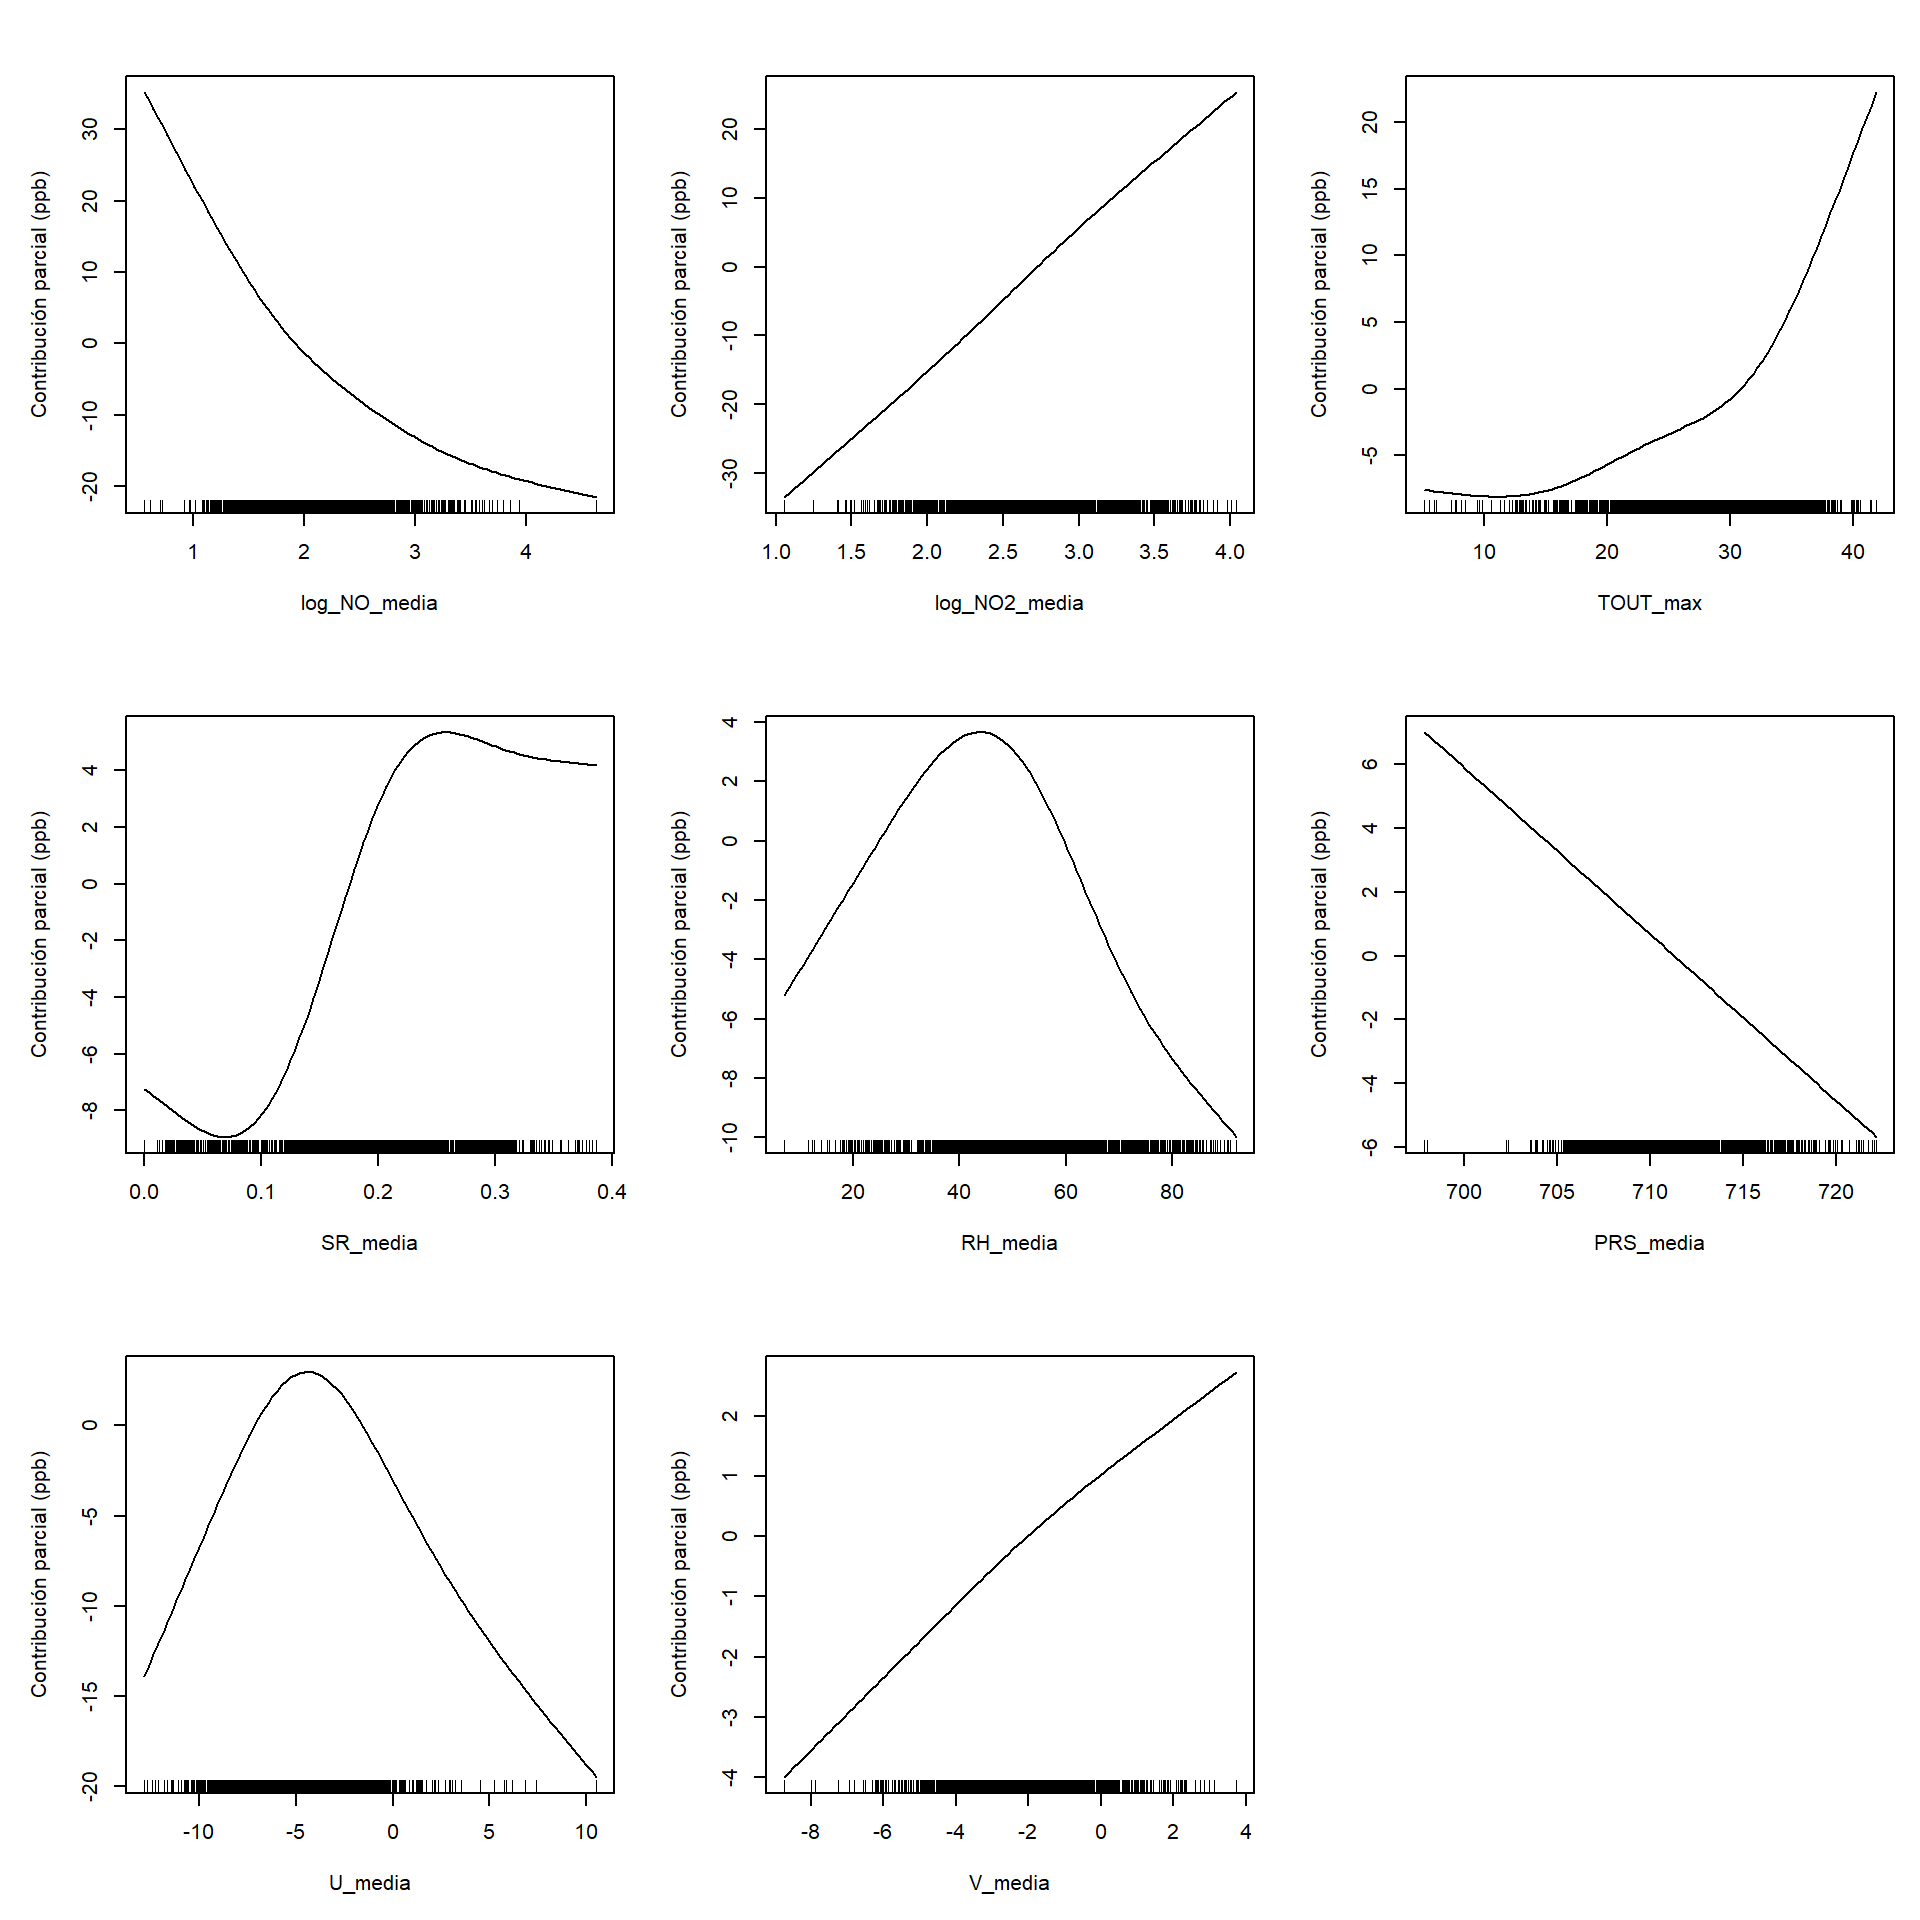
\includegraphics[width=0.97\textwidth,trim=0 487pt 0 0,clip]{img/curvas-predictores-ce-1.png}
\caption{Contribuciones parciales de NO, NO$_2$ y temperatura en el GAM de CE, en ppb. Las marcas horizontales indican disponibilidad de datos. Cada panel tiene escala vertical propia. Paneles reutilizados de la Etapa 3; los demás predictores se resumen en la Tabla~\ref{tab:contribuciones}.}\label{fig:curvas}
\end{figure}
En CE, la contribución de NO disminuye al aumentar; la de NO$_2$ crece; la temperatura aumenta más rápido en valores altos; la radiación sube en el intervalo medio y después se estabiliza, y la humedad alcanza su máximo cerca de 40--45\,\%. Las curvas corresponden a una estación y los extremos tienen menor respaldo de datos. El patrón de NO es compatible con procesos de consumo local de ozono descritos en química atmosférica, pero no permite separarlos del tráfico, la mezcla o el transporte \citep{seinfeld2016}.

\textbf{Corrección de la interpretación inicial.} Las amplitudes dependen del rango observado, de las relaciones entre predictores y del ajuste, por lo que no representan porcentajes de varianza explicada, aportes exclusivos ni una demostración de que precursores y temperatura ``pesan lo mismo''. Aunque NO y NO$_2$ están en escala logarítmica, la respuesta del GAM usa enlace identidad y permanece en ppb, de modo que sus contribuciones no se exponencian ni se suman como efectos causales independientes. Además, sin compuestos orgánicos volátiles y un diseño de atribución no puede deducirse qué reducción de emisiones disminuiría el ozono.
\clearpage


\begin{cambio}
\subsection{Variables relevantes y revisión de la forma del logit}
En las regresiones lineales, temperatura y radiación se relacionaron positivamente con el ozono en las 15 estaciones, mientras que NO y humedad lo hicieron negativamente; NO$_2$ fue positivo en 13. La Tabla~\ref{tab:variables_modelos} cuantifica estas asociaciones manteniendo los demás predictores constantes. Presión y viento presentaron signos menos consistentes, por lo que no se les atribuye una relación uniforme en toda la red.

En ambas logísticas estáticas, temperatura y NO$_2$ tuvieron las mayores asociaciones positivas según el cambio intercuartílico, y NO una asociación negativa. Una OR de 6.32 para temperatura a 60\ppb\ multiplica por 6.32 la razón entre la probabilidad de excedencia y la de no excedencia; no multiplica directamente la probabilidad. Los signos de esos tres predictores, radiación y humedad se conservaron al incorporar AR(1), aunque cambió el signo del viento $U$ y las magnitudes dependen del estado temporal.
\end{cambio}
\begin{table}[H]
\begin{cambio}\centering\small
\begin{tabular}{@{}lrrrr@{}}\toprule
Predictor & Lineal (ppb) & OR 60 & OR 51 & GAMM CE (ppb)\\\midrule
NO transformado & -7.65 & 0.42 & 0.46 & 19.26\\
NO$_2$ transformado & 10.16 & 4.73 & 3.78 & 25.62\\
Temperatura & 6.42 & 6.32 & 4.01 & 13.65\\
Radiación & 6.16 & 1.33 & 1.53 & 12.93\\
Humedad & -2.82 & 0.73 & 0.60 & 7.51\\
Presión & 0.00 & 0.97 & 1.17 & 2.99\\
Viento $U$ & -0.34 & 1.17 & 1.23 & 5.04\\
Viento $V$ & 0.17 & 1.13 & 1.08 & 2.08\\
\bottomrule\end{tabular}
\caption{Asociaciones condicionadas. Lineal indica la mediana entre estaciones del cambio estimado al pasar del percentil 25 al 75 del predictor; OR es la razón de momios para ese cambio en la logística estática; GAMM muestra amplitud P10--P90 del término en CE. Las columnas usan medidas distintas y no representan efectos causales ni aportes exclusivos.}\label{tab:variables_modelos}
\end{cambio}
\end{table}
\begin{cambio}
En el GAMM de CE, las mayores amplitudes fueron NO$_2$ (25.62\ppb), NO (19.26), temperatura (13.65) y radiación (12.93). NO conservó una relación decreciente y NO$_2$ y temperatura una creciente; humedad alcanzó su máximo cerca de 44\,\%. Corregir la dependencia temporal no cambió esta interpretación principal del GAM, aunque sí modificó algunas amplitudes.

\textbf{Linealidad en el logit.} Se compararon rectas con curvas, variable por variable y conjuntamente, usando ajuste 2021--2023 y evaluación 2024 (Fig.~\ref{fig:logit_curvatura}, Anexo~\ref{anexo:retro3}). Las curvas individuales de radiación, y de humedad a 51\ppb, mejoraron la pérdida logarítmica con intervalos semanales de la diferencia por debajo de cero. No se considera comprobada la linealidad estricta. Como tratamiento se añadió una logística con curvas en los ocho predictores, conservando las versiones lineales como referencias explícitamente aproximadas. La pérdida de la alternativa conjunta pasó de 0.445 a 0.495 para 60\ppb\ y de 0.525 a 0.547 para 51\ppb\ en 2024, de modo que no justificó reemplazar automáticamente los modelos principales. Estas comparaciones son exploratorias y no equivalen a pruebas con días independientes.
\end{cambio}
\clearpage

% CUERPO, página 10.
\subsection{Clasificación de excedencias y comparación con AR(1)}
Los resultados de 2025 se evaluaron sobre los mismos 3,368 casos completos, con 833 positivos para 60\ppb\ y 1,432 para 51\ppb. La Tabla~\ref{tab:clasificacion} utiliza los cortes elegidos en 2024 por exactitud balanceada, considerando que el umbral más bajo cambia la definición de la clase y requiere su propio modelo y corte.

\begin{table}[!htbp]\centering\small
\begin{tabular}{@{}llrrrrrrr@{}}
\toprule
Umbral & Modelo & Corte & Sens. & Espec. & Prec. & F1 & FP & FN \\
\midrule
60 ppb & Logística & 0.11 & 83.1 & 74.3 & 51.5 & 0.636 & 651 & 141 \\
60 ppb & Logística AR(1) & 0.16 & 86.1 & 74.5 & 52.6 & 0.653 & 647 & 116 \\
\addlinespace
51 ppb & Logística & 0.26 & 76.1 & 81.3 & 75.1 & 0.756 & 362 & 342 \\
51 ppb & Logística AR(1) & 0.36 & 82.8 & 78.8 & 74.3 & 0.783 & 410 & 246 \\
\bottomrule
\end{tabular}
\caption{Clasificación de 2025. Sens., espec. y prec. se expresan en porcentaje; FP y FN indican falsas alarmas y excedencias omitidas, respectivamente. F1 combina sensibilidad y precisión.}\label{tab:clasificacion}
\end{table}

\textbf{Umbral principal de 60\ppb.} La logística original detectó 692 de 833 excedencias (83.1\,\%), con 651 falsas alarmas y 141 omisiones, mientras que la logística AR(1) detectó 717 (86.1\,\%), con 647 falsas alarmas y 116 omisiones. Así, recuperó 25 excedencias adicionales y redujo cuatro falsas alarmas. La precisión pasó de 51.5 a 52.6\,\%, F1 de 0.636 a 0.653 y la exactitud balanceada de 0.787 a 0.803, aunque la mejora conjunta es moderada y casi la mitad de las alertas sigue siendo falsa.

\textbf{Umbral de 51\ppb.} La detección aumentó de 1,090 a 1,186 excedencias, es decir, de 76.1 a 82.8\,\%, mientras que la exactitud balanceada subió de 0.787 a 0.808 y F1 de 0.756 a 0.783. Sin embargo, el costo fue pasar de 362 a 410 falsas alarmas y reducir ligeramente la precisión, de 75.1 a 74.3\,\%. Por tanto, la mejora favorece la detección sin representar una ganancia en todos los indicadores. Además, la precisión entre umbrales no es directamente comparable como si la prevalencia y la tarea fueran iguales.

\begin{table}[!htbp]\centering\small
\begin{tabular}{@{}lrrrrr@{}}\toprule
60 ppb; corte elegido por F1 & Corte & Sens. (\%) & Prec. (\%) & FP & FN\\\midrule
Logística original & 0.15 & 73.1 & 57.1 & 458 & 224\\
Logística AR(1) & 0.35 & 70.0 & 66.0 & 301 & 250\\\bottomrule
\end{tabular}
\caption{Alternativa de corte elegida con F1 en 2024 y conservada para 2025. F1 fue 0.641 en la logística original y 0.679 en AR(1).}\label{tab:f1}
\end{table}

Cambiar el criterio del corte modifica la decisión práctica. Con F1, AR(1) reduce 157 falsas alarmas respecto a la logística original con su propio corte F1, pero pierde 26 detecciones. Comparado con el AR(1) de corte balanceado, el corte F1 ofrece menos falsas alarmas (301 frente a 647) a costa de más omisiones (250 frente a 116). No se recomienda un corte único como óptimo para SIMA sin acordar si preocupa más emitir falsas alarmas o dejar excedencias sin detectar. El corte balanceado queda como resultado principal para mantener el objetivo de detección.

La exactitud balanceada del AR(1) mejoró en nueve de 14 estaciones para cada umbral, pero la mejora no fue uniforme, pues para 60\ppb\ empeoró en cinco y para 51 empeoró en cuatro y empató en una. El detalle se presenta en el Anexo~\ref{anexo:clasificacion} y debe interpretarse considerando que un porcentaje alto en una estación con pocos días o pocas excedencias no tiene el mismo respaldo que en un sitio con cobertura continua.

El resultado favorece conservar AR(1) como la extensión de mayor utilidad para clasificar los días con apoyo de la información previa de cada estación, aunque esta conclusión se limita a los modelos, la información disponible y los periodos comparados en este proyecto.
\clearpage

% CUERPO, página 11.
\subsection{Dependencia residual, calidad y transferencia}
\figura{ar1_dependencia.pdf}{0.97}{Correlación de residuos de Pearson entre fechas separadas exactamente un día en 2025. Los puntos se calculan por estación y modelo; no son la correlación del estado latente. NTE carece de prueba completa.}{fig:dependencia}
La mediana de la correlación residual diaria entre estaciones bajó de 0.253 a 0.026 para 60\ppb\ y de 0.304 a 0.060 para 51\ppb. También disminuyeron las medianas absolutas (0.253 a 0.051 y 0.304 a 0.063), por lo que el cambio no refleja solo una compensación entre signos. A siete días, la mediana absoluta mejoró para 51\ppb\ (0.087 a 0.030), pero no para 60\ppb\ (0.032 a 0.042). Estos resultados respaldan una menor persistencia diaria sin demostrar la eliminación de toda dependencia.

Los cuatro ajustes AR(1) convergieron con hessiano positivo y parámetros finales $\phi$ cercanos a 0.988 para ambos umbrales. Estos describen persistencia latente en escala logit y no correlaciones de errores binarios. Las comprobaciones de cálculo, filtrado sin respuestas futuras y estabilidad numérica se resumen en el Anexo~\ref{anexo:clasificacion}.

\textbf{Transformación de precursores.} Frente a NO y NO$_2$ sin transformar, los logaritmos mejoraron la precisión de la logística (51.5 frente a 46.7\,\% para 60\ppb; 75.1 frente a 73.2\,\% para 51\ppb) y redujeron el RMSE del GAM en ocho de 14 estaciones. Se conservaron, aunque esta comparación con datos de 2025 no demuestra una ventaja universal.

\textbf{Auditoría de medición.} Se detectaron 2,383 estación--días con radiación nula de 10 a 16 horas en todas las mediciones disponibles (al menos cinco), distintos de los ceros nocturnos esperables. Aunque el socio confirmó fallas de sensores, no indicó fechas afectadas, por lo que las banderas señalan posibles errores, pendientes de confirmación por día. La humedad baja también sigue pendiente de verificación.


\begin{cambio}
En los mismos 3,028 casos sin banderas, filtrar el entrenamiento de la logística estática de 60\ppb\ redujo la detección de 85.1 a 81.4\,\% y elevó la precisión de 50.9 a 54.0\,\%. Tampoco el AR(1) mejoró uniformemente con el filtrado (Anexo~\ref{anexo:retro3}). En NO2, las banderas afectaron los 188 casos de prueba e impidieron una evaluación limpia del GAM.
\end{cambio}


\textbf{Estación nueva.} La validación de estación excluida usó una logística estática complementaria \emph{sin el factor estación} para clasificar sitios no observados, y alcanzó sensibilidad/precisión de 75.0/47.7\,\% para 60\ppb\ y 73.3/69.5\,\% para 51\ppb\ (exactitud balanceada 0.740 y 0.747). El deterioro frente a estaciones conocidas evidencia límites de transferencia, aunque no valida el AR(1) en estaciones nuevas ni aísla un efecto geográfico, pues cambia también la especificación del modelo.
\par

\clearpage

\begin{cambio}
\subsection{Estabilidad temporal, referencia de persistencia e incertidumbre}
La validación repetida mostró que el resultado no es constante entre años (Tabla~\ref{tab:validacion_repetida}). Para 60\ppb, la logística original detectó 75.2, 61.1 y 83.1\,\% de las excedencias en 2023, 2024 y 2025, respectivamente. La precisión también cambió, junto con la frecuencia de excedencias. En los primeros cortes se excluyeron estaciones sin datos para estimar su intercepto inicial; NO3 no entra en la prueba logística de 2023. Las concentraciones también se reevaluaron por año (Anexo~\ref{anexo:retro3}), sin atribuir al AR(1) una validación multianual que no se realizó.
\end{cambio}
\begin{table}[H]
\begin{cambio}\centering\small
\begin{tabular}{@{}lrrrrrrr@{}}\toprule
Prueba & ppb & Casos & Detección (\%) & Precisión (\%) & EB lineal & EB curvas & EB persist.\\\midrule
2023 & 60 & 4334 & 75.2 & 28.1 & 0.752 & 0.766 & 0.736\\
2024 & 60 & 4195 & 61.1 & 49.7 & 0.724 & 0.735 & 0.729\\
2025 & 60 & 3368 & 83.1 & 51.5 & 0.787 & 0.775 & 0.694\\
2023 & 51 & 4334 & 72.4 & 45.4 & 0.729 & 0.735 & 0.722\\
2024 & 51 & 4195 & 57.1 & 75.2 & 0.730 & 0.758 & 0.780\\
2025 & 51 & 3368 & 76.1 & 75.1 & 0.787 & 0.799 & 0.735\\
\bottomrule\end{tabular}
\caption{Validación con ventana de entrenamiento creciente. Para probar el año indicado se selecciona el corte en el año anterior, con ajuste hasta dos años antes, y luego se reajusta hasta el año previo. EB es exactitud balanceada. Se comparan los mismos días y estaciones conocidas por el ajuste inicial de cada corte.}\label{tab:validacion_repetida}
\end{cambio}
\end{table}
\begin{cambio}
\textbf{Referencia de persistencia.} Se clasificó cada día según la excedencia del día calendario anterior en su estación. Si faltó esa observación se usó la frecuencia de entrenamiento, con corte 0.5 (69 casos en 2025). Ese año detectó 53.7\,\% de las excedencias de 60\ppb\ y 69.1\,\% de las de 51\ppb. El AR(1) tuvo mayor EB en ambos umbrales, aunque a 60\ppb\ generó más falsas alarmas (647 frente a 375) y omitió menos excedencias (116 frente a 386). En 2024, la persistencia superó en EB a la logística estática para 51\ppb.
\end{cambio}
\begin{table}[H]
\begin{cambio}\centering\small
\begin{tabular}{@{}lrrrr@{}}\toprule
ppb & Modelo & Detección (\%) & Precisión (\%) & EB\\\midrule
60 & Original & 83.1 [77.2, 88.7] & 51.5 [44.0, 58.9] & 0.787 [0.757, 0.814]\\
60 & AR(1) & 86.1 [81.4, 90.2] & 52.6 [45.1, 59.2] & 0.803 [0.773, 0.828]\\
51 & Original & 76.1 [69.2, 83.1] & 75.1 [69.3, 80.1] & 0.787 [0.755, 0.816]\\
51 & AR(1) & 82.8 [79.0, 86.7] & 74.3 [68.7, 79.0] & 0.808 [0.783, 0.830]\\
\bottomrule\end{tabular}
\caption{Estimación e intervalo percentil del 95\,\% en 2025, con 2,000 remuestreos de bloques móviles de siete días y todas las estaciones juntas. Los intervalos son condicionales a los modelos y cortes ya ajustados.}\label{tab:intervalos_semanales}
\end{cambio}
\end{table}
\begin{cambio}
Los bloques conservan juntas las estaciones y días cercanos. Para ambos umbrales, el intervalo de la diferencia de EB entre AR(1) y original incluye cero, tanto con bloques de siete como de 14 días (Anexo~\ref{anexo:retro3}). La mejora observada no es una ventaja concluyente. Estos intervalos no incluyen incertidumbre de reajuste ni garantizan el desempeño en otro año.
\end{cambio}
\clearpage

% CUERPO, página 12.
\section{Discusión y conclusiones}
\subsection{Respuesta a la pregunta y cumplimiento de los objetivos}

\begin{cambio}
Los datos de SIMA permitieron caracterizar patrones del ozono, cuantificar sus asociaciones y evaluar la clasificación en años posteriores, cumpliendo el objetivo analítico del proyecto. Los resultados no validan un sistema de alerta anticipada ni una explicación causal completa de la contaminación.
\end{cambio}


El primer objetivo específico se refleja en el gradiente de mayor ozono en el poniente, el ciclo con máximos en primavera y otoño y el aumento descriptivo de excedencias de 2024--2025 con umbral constante. Estos resultados conservan la información mejor sustentada de la exploración, pero no distinguen cuánto del cambio se debe a meteorología, emisiones o selección de días disponibles. La altitud y la posición este--oeste están confundidas; describir un patrón geográfico no basta para atribuirlo a una característica del terreno o una fuente cercana.

El segundo objetivo se alcanzó al resumir ocho predictores en cuatro componentes que explican 81.02\,\% de su variación. El PCA identificó ejes relacionados con temperatura/radiación, precursores/humedad y viento, y mostró estabilidad ante las banderas iniciales. Sin embargo, esta síntesis no identifica mecanismos fotoquímicos ni prueba capacidad de clasificación, que se evaluó con los modelos supervisados.


\begin{cambio}
Para el tercer objetivo, el GAM redujo el RMSE de 2025 frente a la regresión lineal en 13 estaciones, en consonancia con la utilidad de modelos flexibles descrita por \citet{laban2020} y \citet{gao2022}. Sin embargo, la revisión multianual mostró estimaciones muy inestables en NO3 al entrenar con solo 46 días antes de 2024. La cobertura y el año evaluado condicionan el resultado; además, mejorar el error medio no evita subestimar días altos. La pequeña ganancia del GAMM de CE tampoco garantiza mejoras importantes al incorporar dependencia temporal.
\end{cambio}



\begin{cambio}
La lectura conjunta de regresión lineal, GAM, GAMM y logística conecta ambos objetivos. Temperatura y NO$_2$ se asociaron con concentraciones y probabilidades mayores, mientras que NO mostró una relación negativa al considerar las demás variables. Esta coincidencia respalda su utilidad analítica, pero no demuestra causalidad, igual importancia ni el efecto de reducir emisiones. El GAM mejora la estimación media sin evitar la subestimación de días altos, mientras que la logística evalúa directamente su clasificación. La ausencia de compuestos orgánicos volátiles limita la explicación química.
\end{cambio}


El cuarto objetivo se cumplió al clasificar ambos umbrales y valorar explícitamente la persistencia. Para 60\ppb, AR(1) detectó 86.1\,\% de las excedencias frente al 83.1\,\% de la logística original y mantuvo prácticamente las falsas alarmas. Para 51\ppb, la detección subió de 76.1 a 82.8\,\%, con más falsas alarmas. La disminución de la dependencia residual diaria respalda el ajuste temporal, pero no transforma por sí sola una precisión de 52.6\,\% en una clasificación suficientemente confiable para automatizar decisiones con consecuencias importantes.

Finalmente, las pruebas de calidad y de estación excluida atendieron el quinto objetivo al mostrar que el desempeño depende del sitio, de la cobertura y de las reglas de inclusión. Así, la evidencia es más sólida en las estaciones con series extensas y continuas, mientras que los resultados de NE, NO3 y SO requieren cautela por su escasa prueba, y NTE permanece sin evaluación posterior completa.

\subsection{Limitaciones que condicionan la interpretación}

\begin{cambio}
La principal limitación de validación es que los años evaluados ya se conocían desde la exploración. Los cortes repetidos muestran variación entre años y los intervalos semanales reconocen dependencia temporal y entre estaciones, pero no crean un periodo ajeno a las decisiones del proyecto. Los intervalos corresponden a predicciones fijas y no incluyen incertidumbre del reajuste. Además, la logística lineal sigue siendo una aproximación, pues el diagnóstico encontró ventajas de curvas individuales sin una mejora uniforme de la alternativa flexible conjunta. No se afirma superioridad general ni eliminación de toda dependencia.
\end{cambio}

\clearpage

% CUERPO, página 13.


\begin{cambio}
La selección de casos completos es otra limitación, pues solo cubren 71.8\,\% del periodo. Entre los 5,263 registros con ozono pero predictores incompletos, 18.3\,\% superó 60\ppb, frente a 16.5\,\% de los completos. La cobertura varió de 59.7\,\% en enero a 78.1\,\% en abril. Estas diferencias advierten un posible sesgo, sin corregirlo. Las banderas meteorológicas requieren confirmación de SIMA, especialmente en NO2.
\end{cambio}


La tercera limitación es de uso, ya que los modelos requieren variables del día objetivo y el AR(1) utiliza, además, respuestas previas verificadas de cada estación. Por tanto, sus resultados muestran cómo se clasifican días pasados aprovechando la información disponible hasta cada fecha, mientras que la validación de transferencia solo se realizó con una logística estática sin interceptos específicos. Aún no se probó una operación con información disponible antes de la jornada ni se cuantificó el efecto de retrasos, ausencia de observaciones o cambios en sensores.

\subsection{Recomendaciones y preguntas abiertas}
A partir de estos resultados se recomiendan las siguientes acciones:
\begin{enumerate}
\setlength{\itemsep}{4pt}
\item \textbf{Priorizar el registro y la revisión de las mediciones.} Contrastar con SIMA las fechas de radiación diurna nula, posibles cambios de escala y humedad extrema; conservar las banderas hasta obtener confirmación. Una mejora de cobertura y calibración puede ser más útil que aumentar la complejidad del modelo.
\item \textbf{Conservar una comparación clara de referencia.} Mantener la logística original junto con AR(1) para documentar el valor de la persistencia. Presentar simultáneamente sensibilidad, precisión y conteos de falsas alarmas, por umbral y estación; no comunicar solo el porcentaje de detección.
\item \textbf{Acordar el propósito de la clasificación.} Si se busca omitir menos excedencias, el corte balanceado ofrece el resultado principal. Si se busca reducir falsas alarmas, la alternativa F1 muestra una opción con menor detección. El criterio final debe responder al costo de los errores y validarse antes de su uso.
\item \textbf{Realizar una prueba futura con decisiones fijadas.} Congelar predictores, parámetros de preparación y regla de corte antes de evaluar un periodo posterior no examinado. Para un pronóstico, utilizar exclusivamente información disponible antes del día objetivo y evaluar también la continuidad del historial requerido por AR(1).
\item \textbf{Ampliar la información ambiental.} Incorporar mediciones de compuestos orgánicos volátiles, inventarios de emisiones y variables de mezcla/transporte cuando estén disponibles. Esto permitiría plantear preguntas de mecanismos y atribución que las asociaciones actuales no resuelven.
\end{enumerate}

Las preguntas que surgen son: ¿la subestimación de 2025 persistirá en un nuevo año con sensores validados? ¿Qué parte del gradiente poniente--oriente corresponde al transporte y cuál a las emisiones locales? ¿Cuánta mejora aporta la historia de ozono o de excedencias frente a la especificación latente elegida? ¿Se mantiene el desempeño al predecir con anticipación y sin respuestas del periodo objetivo? ¿Cómo cambian los resultados al definir episodios de varios días, con reglas explícitas de inicio, duración y separación?


\begin{cambio}
Los precursores y la meteorología ayudaron a describir el ozono mediante PCA y modelos de concentración, aunque el GAM siguió subestimando días altos. La logística evaluó directamente las excedencias y el AR(1) mejoró moderadamente los resultados de 2025; sin embargo, los intervalos por bloques impiden afirmar una ventaja concluyente. El proyecto aporta evidencia para el análisis de SIMA dentro de ese alcance.
\end{cambio}

\label{fin:cuerpo}
\clearpage

\begin{thebibliography}{99}

\bibitem[Brooks et al.(2017)]{brooks2017}
Brooks, M. E., Kristensen, K., van Benthem, K. J., Magnusson, A., Berg, C. W., Nielsen, A., Skaug, H. J., Mächler, M., \& Bolker, B. M. (2017). glmmTMB balances speed and flexibility among packages for zero-inflated generalized linear mixed modeling. \textit{The R Journal, 9}(2), 378--400. \url{https://doi.org/10.32614/RJ-2017-066}

\bibitem[Chang et al.(2025)]{chang2025}
Chang, K.-L., McDonald, B. C., Harkins, C., \& Cooper, O. R. (2025). Surface ozone trend variability across the United States and the impact of heat waves (1990--2023). \textit{Atmospheric Chemistry and Physics, 25}(10), 5101--5132. \url{https://doi.org/10.5194/acp-25-5101-2025}

\bibitem[Gao et al.(2022)]{gao2022}
Gao, Z., Wang, Y., Vasilakos, P., Ivey, C. E., Do, K., \& Russell, A. G. (2022). Predicting peak daily maximum 8 h ozone and linkages to emissions and meteorology in Southern California using machine learning methods (SoCAB-8HR V1.0). \textit{Geoscientific Model Development, 15}(24), 9015--9029. \url{https://doi.org/10.5194/gmd-15-9015-2022}

\bibitem[Iglesias-Gonzalez et al.(2020)]{iglesias2020}
Iglesias-Gonzalez, S., Huertas-Bolanos, M. E., Hernandez-Paniagua, I. Y., \& Mendoza, A. (2020). Explicit modeling of meteorological explanatory variables in short-term forecasting of maximum ozone concentrations via a multiple regression time series framework. \textit{Atmosphere, 11}(12), Article 1304. \url{https://doi.org/10.3390/atmos11121304}

\bibitem[Kristensen \& McGillycuddy(2023)]{glmmtmb}
Kristensen, K., \& McGillycuddy, M. (2023, 14 de octubre). \textit{Covariance structures with glmmTMB} [Documentación técnica]. \url{https://glmmtmb.github.io/glmmTMB/articles/covstruct.html}

\bibitem[Laban et al.(2020)]{laban2020}
Laban, T. L., van Zyl, P. G., Beukes, J. P., Mikkonen, S., Santana, L., Josipovic, M., Vakkari, V., Thompson, A. M., Kulmala, M., \& Laakso, L. (2020). Statistical analysis of factors driving surface ozone variability over continental South Africa. \textit{Journal of Integrative Environmental Sciences, 17}(3), 1--28. \url{https://doi.org/10.1080/1943815X.2020.1768550}

\bibitem[Núñez-Alonso et al.(2019)]{nunez2019}
Núñez-Alonso, D., Pérez-Arribas, L. V., Manzoor, S., \& Cáceres, J. O. (2019). Statistical tools for air pollution assessment: Multivariate and spatial analysis studies in the Madrid region. \textit{Journal of Analytical Methods in Chemistry, 2019}, Article 9753927. \url{https://doi.org/10.1155/2019/9753927}

\bibitem[Otero et al.(2016)]{otero2016}
Otero, N., Sillmann, J., Schnell, J. L., Rust, H. W., \& Butler, T. (2016). Synoptic and meteorological drivers of extreme ozone concentrations over Europe. \textit{Environmental Research Letters, 11}(2), Article 024005. \url{https://doi.org/10.1088/1748-9326/11/2/024005}

\bibitem[Secretaría de Salud(2021)]{salud2021}
Secretaría de Salud. (2021, 28 de octubre). \textit{Norma Oficial Mexicana NOM-020-SSA1-2021, Salud ambiental. Criterio para evaluar la calidad del aire ambiente, con respecto al ozono (O$_3$). Valores normados para la concentración de ozono (O$_3$) en el aire ambiente, como medida de protección a la salud de la población}. Diario Oficial de la Federación. \url{https://sidof.segob.gob.mx/notas/docFuente/5633956}

\bibitem[Seinfeld \& Pandis(2016)]{seinfeld2016}
Seinfeld, J. H., \& Pandis, S. N. (2016). \textit{Atmospheric chemistry and physics: From air pollution to climate change} (3.\textordfeminine{} ed.). Wiley.

\bibitem[SIMA(s.f.)]{simarangos}
Sistema Integral de Monitoreo Ambiental. (s.f.). \textit{Rangos de los parámetros del SIMA} [Documento proporcionado por el socio formador].

\bibitem[SIMA(2025)]{simaubicacion}
Sistema Integral de Monitoreo Ambiental. (2025). \textit{Ubicación de las estaciones de monitoreo} [Documento proporcionado por el socio formador].

\bibitem[SINAICA(s.f.)]{sinaica}
Sistema Nacional de Información de la Calidad del Aire. (s.f.). \textit{Normas Oficiales Mexicanas de salud ambiental}. Instituto Nacional de Ecología y Cambio Climático. Recuperado el 22 de octubre de 2026, de \url{https://sinaica.inecc.gob.mx/pags/noms.php}

\bibitem[Wood(2017)]{wood2017}
Wood, S. N. (2017). \textit{Generalized additive models: An introduction with R} (2.\textordfeminine{} ed.). CRC Press. \url{https://doi.org/10.1201/9781315370279}

\end{thebibliography}
\clearpage

\appendix
\section*{Anexos}
\section{Ubicación, cobertura y asociaciones descriptivas}\label{anexo:datos}
\begin{table}[!htbp]\centering\small
\begin{tabular}{@{}llrrr@{}}\toprule
Estación & Zona & Latitud N & Longitud O & Altitud (m)\\\midrule
SE & Sureste & $25^\circ39'55''$ & $100^\circ14'37''$ & 500\\
NE & Noreste & $25^\circ44'41''$ & $100^\circ15'11''$ & 474\\
CE & Centro & $25^\circ40'33''$ & $100^\circ20'18''$ & 562\\
NO & Noroeste & $25^\circ45'46''$ & $100^\circ22'09''$ & 568\\
SO & Suroeste & $25^\circ40'32''$ & $100^\circ27'29''$ & 674\\
NO2 & Noroeste 2 & $25^\circ48'01''$ & $100^\circ35'04''$ & 702\\
NTE & Norte & $25^\circ47'55''$ & $100^\circ19'38''$ & 503\\
NE2 & Noreste 2 & $25^\circ46'38''$ & $100^\circ11'17''$ & 432\\
SE2 & Sureste 2 & $25^\circ38'45''$ & $100^\circ05'43''$ & 387\\
SO2 & Suroeste 2 & $25^\circ39'54''$ & $100^\circ24'46''$ & 636\\
SE3 & Sureste 3 & $25^\circ36'04''$ & $99^\circ59'57''$ & 334\\
SUR & Sur & $25^\circ37'01''$ & $100^\circ16'26''$ & 555\\
NTE2 & Norte 2 & $25^\circ43'47''$ & $100^\circ18'36''$ & 520\\
NE3 & Noreste 3 & $25^\circ47'26''$ & $100^\circ04'42''$ & 346\\
NO3 & Noroeste 3 & $25^\circ46'06''$ & $100^\circ27'49''$ & 607\\\bottomrule
\end{tabular}
\caption{Ubicación de las estaciones de SIMA según \citet{simaubicacion}.}\label{tab:ubicacion}
\end{table}
\figura{figA1_cobertura.pdf}{0.80}{Cobertura por estación y año, tomada de la Etapa 2. Esta figura usa la definición más amplia de casos completos de aquella etapa (19,585 en 2021--2025), por lo que difiere de los 19,668 del modelo final.}{fig:cobertura}
La disponibilidad de datos explica por qué cada análisis no incluye todos los días posibles. Las regresiones solo requieren las variables de la Tabla~\ref{tab:variables}, por lo que no se exige contar con \NOx\ o temperatura media cuando estas variables no forman parte del modelo.
\clearpage

\figura{fig3_asociaciones.pdf}{0.98}{Asociaciones descriptivas de la Etapa 2, calculadas después de restar a cada variable la media de su estación. Se muestran (a) las diferencias estandarizadas de medias entre días con y sin excedencia de 60 ppb y (b) las correlaciones de Spearman con ozono.}{fig:asociaciones}
% REUTILIZADO: Etapa 2, asociaciones, sin recomendación automática de QDA.
En cada estación, los días con excedencia son principalmente más calurosos ($d=0.90$), más secos ($d=-0.66$), de presión relativamente baja ($d=-0.58$) y más soleados ($d=0.53$). Las diferencias en los precursores son menores entre ambos grupos, pues NO$_2$ y \NOx\ matutino son algo mayores ($d\approx0.3$), mientras que el NO casi no cambia. Las correlaciones con ozono son 0.44 con temperatura, 0.41 con radiación, $-0.45$ con humedad, $-0.30$ con presión y menores de 0.16 en valor absoluto con los precursores y el viento. Estos resultados describen asociaciones, pero no prueban la capacidad de clasificación ni estiman efectos al considerar simultáneamente las demás variables.

\section{Comparación completa de modelos de concentración}\label{anexo:modelos}
\begin{table}[!htbp]\centering\small
\begin{tabular}{@{}lrrrrr@{}}
\toprule
Estación & Días & Ref. mensual & Lineal & GAM & Sesgo GAM \\
\midrule
CE & 308 & 18.28 & 16.42 & \textbf{15.09} & -9.77 \\
NE & 24 & 14.49 & 14.89 & \textbf{13.93} & -7.79 \\
NE2 & 186 & 13.14 & 14.06 & \textbf{12.49} & -5.42 \\
NE3 & 225 & 15.39 & \textbf{8.57} & 9.19 & -0.17 \\
NO & 264 & 17.21 & 15.63 & \textbf{14.46} & -8.39 \\
NO2 & 188 & 22.64 & 20.14 & \textbf{17.12} & -10.57 \\
NO3 & 136 & 21.31 & 14.59 & \textbf{13.37} & -9.24 \\
NTE2 & 344 & 16.66 & 11.20 & \textbf{9.95} & -0.62 \\
SE & 345 & 17.37 & 12.41 & \textbf{11.55} & -3.75 \\
SE2 & 248 & 13.34 & 11.21 & \textbf{10.34} & -3.39 \\
SE3 & 342 & 14.89 & 10.95 & \textbf{10.85} & -5.78 \\
SO & 100 & 17.75 & 12.95 & \textbf{11.85} & -5.24 \\
SO2 & 358 & 18.91 & 12.49 & \textbf{12.04} & -5.89 \\
SUR & 300 & 19.24 & 15.06 & \textbf{14.52} & -6.57 \\
\bottomrule
\end{tabular}
\caption{RMSE y sesgo de 2025 por estación, en ppb. La negrita señala el menor RMSE entre las tres opciones de cada fila. NTE no tiene casos completos de prueba. Las cifras de la Etapa 3 se comprobaron con las predicciones del código actual.}\label{tab:gamcompleto}
\end{table}
Como la disponibilidad de datos cambia entre estaciones, las filas no deben interpretarse como una clasificación de su calidad. Los modelos se compararon con la media mensual de ozono de 2021--2024 de cada estación, y las tres opciones se evaluaron en los mismos días de cada comparación.
\clearpage

\section{Clasificación por estación y verificaciones complementarias}\label{anexo:clasificacion}
\begin{table}[!htbp]\centering\scriptsize
\begin{tabular}{@{}lrrrrrr@{}}
\toprule
 & \multicolumn{3}{c}{60 ppb (logística / AR(1))} & \multicolumn{3}{c}{51 ppb (logística / AR(1))} \\
\cmidrule(lr){2-4}\cmidrule(l){5-7}
Estación & Sens. (\%) & Prec. (\%) & EB & Sens. (\%) & Prec. (\%) & EB \\
\midrule
CE & 89 / 84 & 57 / 54 & 0.789 / 0.754 & 76 / 88 & 79 / 80 & 0.767 / 0.823 \\
NE & 14 / 71 & 100 / 45 & 0.571 / 0.681 & 25 / 67 & 100 / 62 & 0.625 / 0.625 \\
NE2 & 30 / 40 & 50 / 29 & 0.641 / 0.672 & 30 / 52 & 67 / 61 & 0.636 / 0.731 \\
NE3 & 70 / 88 & 64 / 55 & 0.802 / 0.857 & 67 / 77 & 78 / 70 & 0.781 / 0.792 \\
NO & 82 / 86 & 46 / 52 & 0.651 / 0.717 & 83 / 85 & 74 / 75 & 0.711 / 0.725 \\
NO2 & 72 / 90 & 62 / 62 & 0.736 / 0.790 & 58 / 87 & 83 / 84 & 0.705 / 0.815 \\
NO3 & 78 / 88 & 58 / 49 & 0.769 / 0.744 & 89 / 93 & 82 / 77 & 0.833 / 0.797 \\
NTE2 & 87 / 76 & 35 / 40 & 0.782 / 0.773 & 72 / 72 & 62 / 60 & 0.761 / 0.752 \\
SE & 89 / 87 & 47 / 52 & 0.793 / 0.818 & 84 / 77 & 61 / 67 & 0.770 / 0.777 \\
SE2 & 80 / 88 & 62 / 58 & 0.854 / 0.876 & 70 / 75 & 79 / 73 & 0.810 / 0.815 \\
SE3 & 77 / 80 & 57 / 56 & 0.843 / 0.852 & 61 / 77 & 87 / 77 & 0.791 / 0.847 \\
SO & 88 / 85 & 44 / 44 & 0.746 / 0.734 & 91 / 84 & 71 / 68 & 0.801 / 0.759 \\
SO2 & 95 / 92 & 51 / 55 & 0.731 / 0.753 & 89 / 90 & 75 / 78 & 0.746 / 0.781 \\
SUR & 84 / 89 & 56 / 53 & 0.752 / 0.744 & 80 / 88 & 83 / 76 & 0.804 / 0.771 \\
\bottomrule
\end{tabular}

\caption{Clasificación de 2025 por estación, con cortes elegidos por exactitud balanceada (EB). Cada celda muestra logística original / AR(1). NA indica que el valor no puede calcularse porque no hay alertas o falta alguna de las clases.}\label{tab:ar1estaciones}
\end{table}

La EB mejora en nueve estaciones para cada umbral. El número de casos de prueba es CE 308, NE 24, NE2 186, NE3 225, NO 264, NO2 188, NO3 136, NTE2 344, SE 345, SE2 248, SE3 342, SO 100, SO2 358 y SUR 300. NTE no se incluye porque no tiene casos completos de 2025.

\begin{table}[!htbp]\centering\small
\begin{tabular}{@{}rrrrrr@{}}\toprule
Umbral & Ajuste hasta & Casos ajuste & Casos evaluación & $\phi$ & Gradiente máx.\\\midrule
60 & 2023 & 12,105 & 4,195 & 0.9866 & 0.00109\\
60 & 2024 & 16,300 & 3,368 & 0.9885 & 0.00035\\
51 & 2023 & 12,105 & 4,195 & 0.9858 & 0.00517\\
51 & 2024 & 16,300 & 3,368 & 0.9881 & 0.00069\\\bottomrule
\end{tabular}
\caption{Comprobación de los ajustes binomiales con AR(1). Todos convergieron, con hessiano positivo y gradiente máximo menor de 0.01.}\label{tab:controlar1}
\end{table}

El filtrado se comprobó modificando respuestas futuras y verificando que las probabilidades de los días anteriores no cambiaran. También se cambió el orden de las filas para confirmar que no afectara los resultados. Además, se comparó el cálculo con 401 puntos de integración frente a 801 y un intervalo de estados más amplio. Las diferencias máximas entre probabilidades fueron menores de $4\times10^{-15}$ y las clasificaciones no cambiaron. Estas revisiones evalúan el funcionamiento del código, pero no demuestran que el estado AR(1) con distribución normal sea el único proceso temporal adecuado.

Para revisar cómo influye la calidad de los datos, se retiraron del entrenamiento los días con radiación media $>0.4$ kW/m$^2$, humedad $<10$\,\% o ceros diurnos persistentes. Los modelos se compararon en los mismos casos de 2025 sin datos señalados. Para 60\ppb, FP bajó de 606 a 511 y FN subió de 110 a 137; para 51\ppb, la sensibilidad bajó de 79.4 a 75.5\,\% y la precisión subió de 74.4 a 76.4\,\%. La prueba no mejoró todos los resultados ni justifica descartar observaciones sin revisión técnica.

La comparación no mostró una ventaja general de usar los precursores sin transformar, ya que los GAM con $\log(1+x)$ tuvieron menor RMSE en ocho de 14 estaciones. En NO3, el RMSE pasó de 13.71 a 13.37\ppb, aunque sus 332 días de ajuste y 136 de evaluación siguen siendo pocos. En la prueba que dejó una estación fuera del entrenamiento se realizaron 30 ajustes (15 sitios y dos umbrales). Se pudieron evaluar resultados en 14 estaciones, porque NTE no tiene casos de prueba.
\clearpage


\begin{cambio}
\section{Diagnósticos y ampliaciones de la revisión final}\label{anexo:retro3}
La forma del logit se revisó con curvas cúbicas naturales de tres grados de libertad, primero para cada predictor y después para todos juntos. Los nudos de las curvas se fijaron con los datos de entrenamiento de 2021--2023 y se evaluó la pérdida logarítmica en 2024. Esta medida es menor cuando las probabilidades calculadas se acercan más a los resultados observados. El diagnóstico no se basa en la normalidad de los predictores.
\end{cambio}
\begin{table}[H]
\begin{cambio}\centering\small
\begin{tabular}{@{}lrr@{}}\toprule
Predictor con curva & $\Delta$ pérdida 60 ppb & $\Delta$ pérdida 51 ppb\\\midrule
NO transformado & -0.002 [-0.005, 0.002] & -0.001 [-0.006, 0.002]\\
NO$_2$ transformado & 0.026 [0.012, 0.044] & 0.025 [0.013, 0.041]\\
Temperatura & -0.004 [-0.007, 0.000] & -0.004 [-0.008, 0.000]\\
Radiación & -0.008 [-0.013, -0.003] & -0.006 [-0.012, -0.000]\\
Humedad & 0.001 [-0.007, 0.008] & -0.012 [-0.020, -0.004]\\
Presión & 0.005 [0.003, 0.007] & 0.003 [0.002, 0.004]\\
Viento $U$ & 0.010 [-0.005, 0.029] & 0.003 [-0.012, 0.023]\\
Viento $V$ & 0.012 [0.005, 0.019] & 0.007 [0.002, 0.012]\\
Todas las curvas & 0.050 [0.023, 0.083] & 0.022 [-0.005, 0.056]\\
\bottomrule\end{tabular}
\caption{Revisión de la forma de las relaciones. A la pérdida logarítmica de la alternativa con curvas se le resta la de la logística lineal en 2024. Se incluyen intervalos del 95\,\% calculados con percentiles y bloques de siete días. Un valor negativo favorece la curva. Las comparaciones por variable son exploratorias y no se usan como pruebas independientes ni para seleccionar variables automáticamente.}\label{tab:diagnostico_logit}
\end{cambio}
\end{table}
\begin{cambio}
Las curvas por variable aportaron evidencia de que una recta no describe suficientemente la relación de la radiación y, a 51\ppb, de la humedad. Transformar NO y NO$_2$ no demuestra que las relaciones de los demás predictores sean lineales. Se mantiene la logística lineal como referencia y se presenta la alternativa con curvas, que tampoco mejora de forma uniforme la detección y las falsas alarmas (Tabla~\ref{tab:comparacion_ampliada}). No se añadieron nuevos términos suaves al AR(1) para corregir la forma de esas relaciones, por lo que reducir la dependencia temporal no resuelve esta limitación.

El modelo con curvas de 60\ppb\ usado para evaluar 2023 convergió, aunque generó una advertencia por probabilidades cercanas a cero o uno. Usar un modelo más flexible con pocos datos previos requiere precaución y no garantiza una mejora.
\end{cambio}
\begin{table}[H]
\begin{cambio}\centering\small
\begin{tabular}{@{}lrrrrrr@{}}\toprule
ppb & Modelo & Detección (\%) & Precisión (\%) & FP & FN & EB\\\midrule
60 & Original & 83.1 & 51.5 & 651 & 141 & 0.787\\
60 & AR(1) & 86.1 & 52.6 & 647 & 116 & 0.803\\
60 & Logística con curvas & 89.2 & 46.1 & 867 & 90 & 0.775\\
60 & Persistencia & 53.7 & 54.4 & 375 & 386 & 0.694\\
51 & Original & 76.1 & 75.1 & 362 & 342 & 0.787\\
51 & AR(1) & 82.8 & 74.3 & 410 & 246 & 0.808\\
51 & Logística con curvas & 84.8 & 71.4 & 486 & 217 & 0.799\\
51 & Persistencia & 69.1 & 69.7 & 429 & 443 & 0.735\\
\bottomrule\end{tabular}
\caption{Comparación ampliada de la clasificación de 2025 en los mismos 3,368 estación--días. Los cortes de las logísticas se eligieron en 2024 y la referencia de persistencia usa corte 0.5. El modelo con curvas permite tratar posibles relaciones no lineales, pero no mejora todos los indicadores.}\label{tab:comparacion_ampliada}
\end{cambio}
\end{table}
\begin{cambio}
Para 60\ppb, la logística con curvas aumentó la detección a 89.2\,\%, pero bajó la precisión a 46.1\,\% y produjo 867 falsas alarmas. Para 51\ppb\ mejoró la EB respecto a la logística original, aunque quedó por debajo del AR(1). Por tanto, permitir relaciones curvas no resolvió por sí solo el balance entre falsas alarmas y excedencias omitidas.
\end{cambio}
\clearpage
\begin{figure}[H]
\begin{cambio}\centering%
{\small\textcolor{blue!65!black}{\rule{15pt}{1pt} 60 ppb}\qquad\textcolor{orange!80!black}{\rule{15pt}{1pt} 51 ppb}}\par%
\setlength{\unitlength}{1pt}\begin{picture}(460,455)%
\put(125.00,433.00){\makebox(0,0){\small\bfseries NO transformado}}%
{\color{black!12}\linethickness{0.2pt}\put(35,349.00){\line(1,0){180}}}%
\put(30,349.00){\makebox(0,0)[r]{\scriptsize -1.5}}%
{\color{black!12}\linethickness{0.2pt}\put(35,363.40){\line(1,0){180}}}%
\put(30,363.40){\makebox(0,0)[r]{\scriptsize -1}}%
{\color{black!12}\linethickness{0.2pt}\put(35,377.80){\line(1,0){180}}}%
\put(30,377.80){\makebox(0,0)[r]{\scriptsize -0.5}}%
{\color{black!45}\linethickness{0.4pt}\put(35,392.20){\line(1,0){180}}}%
\put(30,392.20){\makebox(0,0)[r]{\scriptsize 0}}%
{\color{black!12}\linethickness{0.2pt}\put(35,406.60){\line(1,0){180}}}%
\put(30,406.60){\makebox(0,0)[r]{\scriptsize 0.5}}%
{\color{black!12}\linethickness{0.2pt}\put(35,421.00){\line(1,0){180}}}%
\put(30,421.00){\makebox(0,0)[r]{\scriptsize 1}}%
{\linethickness{0.3pt}\put(35,349){\line(1,0){180}}\put(35,349){\line(0,1){72}}}%
\put(35,340){\makebox(0,0){\scriptsize P5}}%
\put(215,340){\makebox(0,0){\scriptsize P95}}%
\put(10,385.0){\makebox(0,0){\rotatebox{90}{\scriptsize Desviación del logit}}}%
{\color{blue!65!black}\linethickness{0.8pt}%
\qbezier(35.00,402.42)(37.73,401.20)(40.45,399.98)%
\qbezier(40.45,399.98)(43.18,398.86)(45.91,397.75)%
\qbezier(45.91,397.75)(48.64,396.74)(51.36,395.74)%
\qbezier(51.36,395.74)(54.09,394.86)(56.82,393.97)%
\qbezier(56.82,393.97)(59.55,393.21)(62.27,392.45)%
\qbezier(62.27,392.45)(65.00,391.83)(67.73,391.20)%
\qbezier(67.73,391.20)(70.45,390.71)(73.18,390.22)%
\qbezier(73.18,390.22)(75.91,389.86)(78.64,389.50)%
\qbezier(78.64,389.50)(81.36,389.25)(84.09,389.00)%
\qbezier(84.09,389.00)(86.82,388.85)(89.55,388.70)%
\qbezier(89.55,388.70)(92.27,388.63)(95.00,388.56)%
\qbezier(95.00,388.56)(97.73,388.56)(100.45,388.56)%
\qbezier(100.45,388.56)(103.18,388.61)(105.91,388.67)%
\qbezier(105.91,388.67)(108.64,388.76)(111.36,388.85)%
\qbezier(111.36,388.85)(114.09,388.97)(116.82,389.09)%
\qbezier(116.82,389.09)(119.55,389.22)(122.27,389.35)%
\qbezier(122.27,389.35)(125.00,389.49)(127.73,389.63)%
\qbezier(127.73,389.63)(130.45,389.78)(133.18,389.93)%
\qbezier(133.18,389.93)(135.91,390.09)(138.64,390.25)%
\qbezier(138.64,390.25)(141.36,390.41)(144.09,390.58)%
\qbezier(144.09,390.58)(146.82,390.76)(149.55,390.94)%
\qbezier(149.55,390.94)(152.27,391.12)(155.00,391.31)%
\qbezier(155.00,391.31)(157.73,391.50)(160.45,391.69)%
\qbezier(160.45,391.69)(163.18,391.89)(165.91,392.09)%
\qbezier(165.91,392.09)(168.64,392.30)(171.36,392.51)%
\qbezier(171.36,392.51)(174.09,392.73)(176.82,392.95)%
\qbezier(176.82,392.95)(179.55,393.17)(182.27,393.39)%
\qbezier(182.27,393.39)(185.00,393.63)(187.73,393.86)%
\qbezier(187.73,393.86)(190.45,394.10)(193.18,394.33)%
\qbezier(193.18,394.33)(195.91,394.58)(198.64,394.82)%
\qbezier(198.64,394.82)(201.36,395.07)(204.09,395.33)%
\qbezier(204.09,395.33)(206.82,395.58)(209.55,395.84)%
\qbezier(209.55,395.84)(212.27,396.10)(215.00,396.37)%
}%
{\color{orange!80!black}\linethickness{0.8pt}%
\qbezier(35.00,403.01)(37.73,401.68)(40.45,400.35)%
\qbezier(40.45,400.35)(43.18,399.14)(45.91,397.92)%
\qbezier(45.91,397.92)(48.64,396.84)(51.36,395.75)%
\qbezier(51.36,395.75)(54.09,394.80)(56.82,393.85)%
\qbezier(56.82,393.85)(59.55,393.04)(62.27,392.23)%
\qbezier(62.27,392.23)(65.00,391.57)(67.73,390.91)%
\qbezier(67.73,390.91)(70.45,390.40)(73.18,389.90)%
\qbezier(73.18,389.90)(75.91,389.53)(78.64,389.17)%
\qbezier(78.64,389.17)(81.36,388.93)(84.09,388.69)%
\qbezier(84.09,388.69)(86.82,388.56)(89.55,388.43)%
\qbezier(89.55,388.43)(92.27,388.39)(95.00,388.35)%
\qbezier(95.00,388.35)(97.73,388.39)(100.45,388.42)%
\qbezier(100.45,388.42)(103.18,388.51)(105.91,388.60)%
\qbezier(105.91,388.60)(108.64,388.73)(111.36,388.86)%
\qbezier(111.36,388.86)(114.09,389.01)(116.82,389.16)%
\qbezier(116.82,389.16)(119.55,389.32)(122.27,389.48)%
\qbezier(122.27,389.48)(125.00,389.64)(127.73,389.81)%
\qbezier(127.73,389.81)(130.45,389.97)(133.18,390.14)%
\qbezier(133.18,390.14)(135.91,390.31)(138.64,390.48)%
\qbezier(138.64,390.48)(141.36,390.65)(144.09,390.83)%
\qbezier(144.09,390.83)(146.82,391.01)(149.55,391.18)%
\qbezier(149.55,391.18)(152.27,391.36)(155.00,391.55)%
\qbezier(155.00,391.55)(157.73,391.73)(160.45,391.92)%
\qbezier(160.45,391.92)(163.18,392.10)(165.91,392.29)%
\qbezier(165.91,392.29)(168.64,392.48)(171.36,392.68)%
\qbezier(171.36,392.68)(174.09,392.87)(176.82,393.07)%
\qbezier(176.82,393.07)(179.55,393.26)(182.27,393.46)%
\qbezier(182.27,393.46)(185.00,393.66)(187.73,393.86)%
\qbezier(187.73,393.86)(190.45,394.07)(193.18,394.27)%
\qbezier(193.18,394.27)(195.91,394.48)(198.64,394.69)%
\qbezier(198.64,394.69)(201.36,394.90)(204.09,395.11)%
\qbezier(204.09,395.11)(206.82,395.32)(209.55,395.53)%
\qbezier(209.55,395.53)(212.27,395.74)(215.00,395.96)%
}%
\put(357.00,433.00){\makebox(0,0){\small\bfseries NO$_2$ transformado}}%
{\color{black!12}\linethickness{0.2pt}\put(267,349.00){\line(1,0){180}}}%
\put(262,349.00){\makebox(0,0)[r]{\scriptsize -1.5}}%
{\color{black!12}\linethickness{0.2pt}\put(267,363.40){\line(1,0){180}}}%
\put(262,363.40){\makebox(0,0)[r]{\scriptsize -1}}%
{\color{black!12}\linethickness{0.2pt}\put(267,377.80){\line(1,0){180}}}%
\put(262,377.80){\makebox(0,0)[r]{\scriptsize -0.5}}%
{\color{black!45}\linethickness{0.4pt}\put(267,392.20){\line(1,0){180}}}%
\put(262,392.20){\makebox(0,0)[r]{\scriptsize 0}}%
{\color{black!12}\linethickness{0.2pt}\put(267,406.60){\line(1,0){180}}}%
\put(262,406.60){\makebox(0,0)[r]{\scriptsize 0.5}}%
{\color{black!12}\linethickness{0.2pt}\put(267,421.00){\line(1,0){180}}}%
\put(262,421.00){\makebox(0,0)[r]{\scriptsize 1}}%
{\linethickness{0.3pt}\put(267,349){\line(1,0){180}}\put(267,349){\line(0,1){72}}}%
\put(267,340){\makebox(0,0){\scriptsize P5}}%
\put(447,340){\makebox(0,0){\scriptsize P95}}%
{\color{blue!65!black}\linethickness{0.8pt}%
\qbezier(267.00,375.28)(269.73,376.78)(272.45,378.28)%
\qbezier(272.45,378.28)(275.18,379.70)(277.91,381.12)%
\qbezier(277.91,381.12)(280.64,382.45)(283.36,383.79)%
\qbezier(283.36,383.79)(286.09,385.03)(288.82,386.28)%
\qbezier(288.82,386.28)(291.55,387.44)(294.27,388.59)%
\qbezier(294.27,388.59)(297.00,389.66)(299.73,390.72)%
\qbezier(299.73,390.72)(302.45,391.69)(305.18,392.66)%
\qbezier(305.18,392.66)(307.91,393.52)(310.64,394.39)%
\qbezier(310.64,394.39)(313.36,395.16)(316.09,395.93)%
\qbezier(316.09,395.93)(318.82,396.60)(321.55,397.26)%
\qbezier(321.55,397.26)(324.27,397.82)(327.00,398.38)%
\qbezier(327.00,398.38)(329.73,398.83)(332.45,399.29)%
\qbezier(332.45,399.29)(335.18,399.63)(337.91,399.97)%
\qbezier(337.91,399.97)(340.64,400.21)(343.36,400.45)%
\qbezier(343.36,400.45)(346.09,400.59)(348.82,400.73)%
\qbezier(348.82,400.73)(351.55,400.77)(354.27,400.80)%
\qbezier(354.27,400.80)(357.00,400.75)(359.73,400.69)%
\qbezier(359.73,400.69)(362.45,400.54)(365.18,400.38)%
\qbezier(365.18,400.38)(367.91,400.14)(370.64,399.90)%
\qbezier(370.64,399.90)(373.36,399.57)(376.09,399.24)%
\qbezier(376.09,399.24)(378.82,398.82)(381.55,398.40)%
\qbezier(381.55,398.40)(384.27,397.90)(387.00,397.40)%
\qbezier(387.00,397.40)(389.73,396.83)(392.45,396.25)%
\qbezier(392.45,396.25)(395.18,395.59)(397.91,394.93)%
\qbezier(397.91,394.93)(400.64,394.20)(403.36,393.47)%
\qbezier(403.36,393.47)(406.09,392.67)(408.82,391.87)%
\qbezier(408.82,391.87)(411.55,391.00)(414.27,390.12)%
\qbezier(414.27,390.12)(417.00,389.19)(419.73,388.25)%
\qbezier(419.73,388.25)(422.45,387.25)(425.18,386.25)%
\qbezier(425.18,386.25)(427.91,385.19)(430.64,384.12)%
\qbezier(430.64,384.12)(433.36,383.00)(436.09,381.88)%
\qbezier(436.09,381.88)(438.82,380.71)(441.55,379.53)%
\qbezier(441.55,379.53)(444.27,378.30)(447.00,377.08)%
}%
{\color{orange!80!black}\linethickness{0.8pt}%
\qbezier(267.00,379.51)(269.73,380.58)(272.45,381.66)%
\qbezier(272.45,381.66)(275.18,382.68)(277.91,383.70)%
\qbezier(277.91,383.70)(280.64,384.67)(283.36,385.63)%
\qbezier(283.36,385.63)(286.09,386.54)(288.82,387.45)%
\qbezier(288.82,387.45)(291.55,388.30)(294.27,389.15)%
\qbezier(294.27,389.15)(297.00,389.93)(299.73,390.72)%
\qbezier(299.73,390.72)(302.45,391.45)(305.18,392.17)%
\qbezier(305.18,392.17)(307.91,392.83)(310.64,393.49)%
\qbezier(310.64,393.49)(313.36,394.09)(316.09,394.68)%
\qbezier(316.09,394.68)(318.82,395.21)(321.55,395.74)%
\qbezier(321.55,395.74)(324.27,396.20)(327.00,396.65)%
\qbezier(327.00,396.65)(329.73,397.04)(332.45,397.43)%
\qbezier(332.45,397.43)(335.18,397.74)(337.91,398.06)%
\qbezier(337.91,398.06)(340.64,398.30)(343.36,398.54)%
\qbezier(343.36,398.54)(346.09,398.71)(348.82,398.87)%
\qbezier(348.82,398.87)(351.55,398.96)(354.27,399.06)%
\qbezier(354.27,399.06)(357.00,399.07)(359.73,399.08)%
\qbezier(359.73,399.08)(362.45,399.02)(365.18,398.96)%
\qbezier(365.18,398.96)(367.91,398.82)(370.64,398.68)%
\qbezier(370.64,398.68)(373.36,398.45)(376.09,398.23)%
\qbezier(376.09,398.23)(378.82,397.93)(381.55,397.63)%
\qbezier(381.55,397.63)(384.27,397.25)(387.00,396.86)%
\qbezier(387.00,396.86)(389.73,396.40)(392.45,395.94)%
\qbezier(392.45,395.94)(395.18,395.41)(397.91,394.87)%
\qbezier(397.91,394.87)(400.64,394.26)(403.36,393.65)%
\qbezier(403.36,393.65)(406.09,392.97)(408.82,392.29)%
\qbezier(408.82,392.29)(411.55,391.54)(414.27,390.79)%
\qbezier(414.27,390.79)(417.00,389.98)(419.73,389.17)%
\qbezier(419.73,389.17)(422.45,388.29)(425.18,387.41)%
\qbezier(425.18,387.41)(427.91,386.48)(430.64,385.54)%
\qbezier(430.64,385.54)(433.36,384.55)(436.09,383.56)%
\qbezier(436.09,383.56)(438.82,382.51)(441.55,381.47)%
\qbezier(441.55,381.47)(444.27,380.37)(447.00,379.27)%
}%
\put(125.00,325.00){\makebox(0,0){\small\bfseries Temperatura}}%
{\color{black!12}\linethickness{0.2pt}\put(35,241.00){\line(1,0){180}}}%
\put(30,241.00){\makebox(0,0)[r]{\scriptsize -1.5}}%
{\color{black!12}\linethickness{0.2pt}\put(35,255.40){\line(1,0){180}}}%
\put(30,255.40){\makebox(0,0)[r]{\scriptsize -1}}%
{\color{black!12}\linethickness{0.2pt}\put(35,269.80){\line(1,0){180}}}%
\put(30,269.80){\makebox(0,0)[r]{\scriptsize -0.5}}%
{\color{black!45}\linethickness{0.4pt}\put(35,284.20){\line(1,0){180}}}%
\put(30,284.20){\makebox(0,0)[r]{\scriptsize 0}}%
{\color{black!12}\linethickness{0.2pt}\put(35,298.60){\line(1,0){180}}}%
\put(30,298.60){\makebox(0,0)[r]{\scriptsize 0.5}}%
{\color{black!12}\linethickness{0.2pt}\put(35,313.00){\line(1,0){180}}}%
\put(30,313.00){\makebox(0,0)[r]{\scriptsize 1}}%
{\linethickness{0.3pt}\put(35,241){\line(1,0){180}}\put(35,241){\line(0,1){72}}}%
\put(35,232){\makebox(0,0){\scriptsize P5}}%
\put(215,232){\makebox(0,0){\scriptsize P95}}%
\put(10,277.0){\makebox(0,0){\rotatebox{90}{\scriptsize Desviación del logit}}}%
{\color{blue!65!black}\linethickness{0.8pt}%
\qbezier(35.00,256.28)(37.73,258.89)(40.45,261.50)%
\qbezier(40.45,261.50)(43.18,263.98)(45.91,266.45)%
\qbezier(45.91,266.45)(48.64,268.78)(51.36,271.12)%
\qbezier(51.36,271.12)(54.09,273.29)(56.82,275.47)%
\qbezier(56.82,275.47)(59.55,277.49)(62.27,279.51)%
\qbezier(62.27,279.51)(65.00,281.36)(67.73,283.21)%
\qbezier(67.73,283.21)(70.45,284.89)(73.18,286.57)%
\qbezier(73.18,286.57)(75.91,288.06)(78.64,289.55)%
\qbezier(78.64,289.55)(81.36,290.85)(84.09,292.16)%
\qbezier(84.09,292.16)(86.82,293.26)(89.55,294.37)%
\qbezier(89.55,294.37)(92.27,295.26)(95.00,296.16)%
\qbezier(95.00,296.16)(97.73,296.85)(100.45,297.53)%
\qbezier(100.45,297.53)(103.18,298.00)(105.91,298.46)%
\qbezier(105.91,298.46)(108.64,298.70)(111.36,298.93)%
\qbezier(111.36,298.93)(114.09,298.93)(116.82,298.93)%
\qbezier(116.82,298.93)(119.55,298.69)(122.27,298.44)%
\qbezier(122.27,298.44)(125.00,297.95)(127.73,297.45)%
\qbezier(127.73,297.45)(130.45,296.71)(133.18,295.96)%
\qbezier(133.18,295.96)(135.91,295.02)(138.64,294.07)%
\qbezier(138.64,294.07)(141.36,292.97)(144.09,291.87)%
\qbezier(144.09,291.87)(146.82,290.67)(149.55,289.47)%
\qbezier(149.55,289.47)(152.27,288.22)(155.00,286.98)%
\qbezier(155.00,286.98)(157.73,285.74)(160.45,284.49)%
\qbezier(160.45,284.49)(163.18,283.31)(165.91,282.13)%
\qbezier(165.91,282.13)(168.64,281.06)(171.36,279.99)%
\qbezier(171.36,279.99)(174.09,279.08)(176.82,278.17)%
\qbezier(176.82,278.17)(179.55,277.44)(182.27,276.72)%
\qbezier(182.27,276.72)(185.00,276.17)(187.73,275.63)%
\qbezier(187.73,275.63)(190.45,275.24)(193.18,274.86)%
\qbezier(193.18,274.86)(195.91,274.63)(198.64,274.40)%
\qbezier(198.64,274.40)(201.36,274.30)(204.09,274.21)%
\qbezier(204.09,274.21)(206.82,274.25)(209.55,274.29)%
\qbezier(209.55,274.29)(212.27,274.44)(215.00,274.59)%
}%
{\color{orange!80!black}\linethickness{0.8pt}%
\qbezier(35.00,267.46)(37.73,269.03)(40.45,270.60)%
\qbezier(40.45,270.60)(43.18,272.08)(45.91,273.57)%
\qbezier(45.91,273.57)(48.64,274.96)(51.36,276.36)%
\qbezier(51.36,276.36)(54.09,277.67)(56.82,278.97)%
\qbezier(56.82,278.97)(59.55,280.18)(62.27,281.39)%
\qbezier(62.27,281.39)(65.00,282.50)(67.73,283.61)%
\qbezier(67.73,283.61)(70.45,284.62)(73.18,285.62)%
\qbezier(73.18,285.62)(75.91,286.52)(78.64,287.41)%
\qbezier(78.64,287.41)(81.36,288.19)(84.09,288.97)%
\qbezier(84.09,288.97)(86.82,289.64)(89.55,290.30)%
\qbezier(89.55,290.30)(92.27,290.84)(95.00,291.37)%
\qbezier(95.00,291.37)(97.73,291.78)(100.45,292.19)%
\qbezier(100.45,292.19)(103.18,292.47)(105.91,292.75)%
\qbezier(105.91,292.75)(108.64,292.89)(111.36,293.03)%
\qbezier(111.36,293.03)(114.09,293.03)(116.82,293.03)%
\qbezier(116.82,293.03)(119.55,292.88)(122.27,292.73)%
\qbezier(122.27,292.73)(125.00,292.44)(127.73,292.14)%
\qbezier(127.73,292.14)(130.45,291.69)(133.18,291.24)%
\qbezier(133.18,291.24)(135.91,290.67)(138.64,290.10)%
\qbezier(138.64,290.10)(141.36,289.44)(144.09,288.78)%
\qbezier(144.09,288.78)(146.82,288.06)(149.55,287.34)%
\qbezier(149.55,287.34)(152.27,286.60)(155.00,285.85)%
\qbezier(155.00,285.85)(157.73,285.10)(160.45,284.36)%
\qbezier(160.45,284.36)(163.18,283.65)(165.91,282.94)%
\qbezier(165.91,282.94)(168.64,282.30)(171.36,281.66)%
\qbezier(171.36,281.66)(174.09,281.12)(176.82,280.57)%
\qbezier(176.82,280.57)(179.55,280.14)(182.27,279.71)%
\qbezier(182.27,279.71)(185.00,279.38)(187.73,279.06)%
\qbezier(187.73,279.06)(190.45,278.83)(193.18,278.60)%
\qbezier(193.18,278.60)(195.91,278.47)(198.64,278.34)%
\qbezier(198.64,278.34)(201.36,278.28)(204.09,278.23)%
\qbezier(204.09,278.23)(206.82,278.26)(209.55,278.29)%
\qbezier(209.55,278.29)(212.27,278.38)(215.00,278.48)%
}%
\put(357.00,325.00){\makebox(0,0){\small\bfseries Radiación}}%
{\color{black!12}\linethickness{0.2pt}\put(267,241.00){\line(1,0){180}}}%
\put(262,241.00){\makebox(0,0)[r]{\scriptsize -1.5}}%
{\color{black!12}\linethickness{0.2pt}\put(267,255.40){\line(1,0){180}}}%
\put(262,255.40){\makebox(0,0)[r]{\scriptsize -1}}%
{\color{black!12}\linethickness{0.2pt}\put(267,269.80){\line(1,0){180}}}%
\put(262,269.80){\makebox(0,0)[r]{\scriptsize -0.5}}%
{\color{black!45}\linethickness{0.4pt}\put(267,284.20){\line(1,0){180}}}%
\put(262,284.20){\makebox(0,0)[r]{\scriptsize 0}}%
{\color{black!12}\linethickness{0.2pt}\put(267,298.60){\line(1,0){180}}}%
\put(262,298.60){\makebox(0,0)[r]{\scriptsize 0.5}}%
{\color{black!12}\linethickness{0.2pt}\put(267,313.00){\line(1,0){180}}}%
\put(262,313.00){\makebox(0,0)[r]{\scriptsize 1}}%
{\linethickness{0.3pt}\put(267,241){\line(1,0){180}}\put(267,241){\line(0,1){72}}}%
\put(267,232){\makebox(0,0){\scriptsize P5}}%
\put(447,232){\makebox(0,0){\scriptsize P95}}%
{\color{blue!65!black}\linethickness{0.8pt}%
\qbezier(267.00,304.47)(269.73,302.68)(272.45,300.88)%
\qbezier(272.45,300.88)(275.18,299.10)(277.91,297.32)%
\qbezier(277.91,297.32)(280.64,295.58)(283.36,293.85)%
\qbezier(283.36,293.85)(286.09,292.17)(288.82,290.49)%
\qbezier(288.82,290.49)(291.55,288.89)(294.27,287.29)%
\qbezier(294.27,287.29)(297.00,285.79)(299.73,284.29)%
\qbezier(299.73,284.29)(302.45,282.90)(305.18,281.52)%
\qbezier(305.18,281.52)(307.91,280.28)(310.64,279.03)%
\qbezier(310.64,279.03)(313.36,277.95)(316.09,276.86)%
\qbezier(316.09,276.86)(318.82,275.95)(321.55,275.05)%
\qbezier(321.55,275.05)(324.27,274.34)(327.00,273.62)%
\qbezier(327.00,273.62)(329.73,273.13)(332.45,272.64)%
\qbezier(332.45,272.64)(335.18,272.38)(337.91,272.13)%
\qbezier(337.91,272.13)(340.64,272.13)(343.36,272.13)%
\qbezier(343.36,272.13)(346.09,272.41)(348.82,272.68)%
\qbezier(348.82,272.68)(351.55,273.25)(354.27,273.81)%
\qbezier(354.27,273.81)(357.00,274.61)(359.73,275.42)%
\qbezier(359.73,275.42)(362.45,276.40)(365.18,277.38)%
\qbezier(365.18,277.38)(367.91,278.47)(370.64,279.56)%
\qbezier(370.64,279.56)(373.36,280.70)(376.09,281.83)%
\qbezier(376.09,281.83)(378.82,282.95)(381.55,284.07)%
\qbezier(381.55,284.07)(384.27,285.10)(387.00,286.13)%
\qbezier(387.00,286.13)(389.73,287.02)(392.45,287.90)%
\qbezier(392.45,287.90)(395.18,288.59)(397.91,289.27)%
\qbezier(397.91,289.27)(400.64,289.75)(403.36,290.23)%
\qbezier(403.36,290.23)(406.09,290.51)(408.82,290.78)%
\qbezier(408.82,290.78)(411.55,290.86)(414.27,290.94)%
\qbezier(414.27,290.94)(417.00,290.83)(419.73,290.72)%
\qbezier(419.73,290.72)(422.45,290.42)(425.18,290.12)%
\qbezier(425.18,290.12)(427.91,289.63)(430.64,289.15)%
\qbezier(430.64,289.15)(433.36,288.48)(436.09,287.82)%
\qbezier(436.09,287.82)(438.82,286.98)(441.55,286.14)%
\qbezier(441.55,286.14)(444.27,285.12)(447.00,284.11)%
}%
{\color{orange!80!black}\linethickness{0.8pt}%
\qbezier(267.00,303.42)(269.73,301.67)(272.45,299.92)%
\qbezier(272.45,299.92)(275.18,298.19)(277.91,296.46)%
\qbezier(277.91,296.46)(280.64,294.77)(283.36,293.07)%
\qbezier(283.36,293.07)(286.09,291.44)(288.82,289.81)%
\qbezier(288.82,289.81)(291.55,288.26)(294.27,286.71)%
\qbezier(294.27,286.71)(297.00,285.26)(299.73,283.81)%
\qbezier(299.73,283.81)(302.45,282.48)(305.18,281.15)%
\qbezier(305.18,281.15)(307.91,279.96)(310.64,278.77)%
\qbezier(310.64,278.77)(313.36,277.74)(316.09,276.71)%
\qbezier(316.09,276.71)(318.82,275.86)(321.55,275.01)%
\qbezier(321.55,275.01)(324.27,274.36)(327.00,273.72)%
\qbezier(327.00,273.72)(329.73,273.29)(332.45,272.86)%
\qbezier(332.45,272.86)(335.18,272.67)(337.91,272.49)%
\qbezier(337.91,272.49)(340.64,272.56)(343.36,272.63)%
\qbezier(343.36,272.63)(346.09,272.99)(348.82,273.34)%
\qbezier(348.82,273.34)(351.55,273.99)(354.27,274.63)%
\qbezier(354.27,274.63)(357.00,275.52)(359.73,276.40)%
\qbezier(359.73,276.40)(362.45,277.45)(365.18,278.51)%
\qbezier(365.18,278.51)(367.91,279.66)(370.64,280.82)%
\qbezier(370.64,280.82)(373.36,282.00)(376.09,283.18)%
\qbezier(376.09,283.18)(378.82,284.32)(381.55,285.47)%
\qbezier(381.55,285.47)(384.27,286.49)(387.00,287.52)%
\qbezier(387.00,287.52)(389.73,288.37)(392.45,289.22)%
\qbezier(392.45,289.22)(395.18,289.83)(397.91,290.44)%
\qbezier(397.91,290.44)(400.64,290.81)(403.36,291.18)%
\qbezier(403.36,291.18)(406.09,291.30)(408.82,291.43)%
\qbezier(408.82,291.43)(411.55,291.33)(414.27,291.23)%
\qbezier(414.27,291.23)(417.00,290.89)(419.73,290.56)%
\qbezier(419.73,290.56)(422.45,290.01)(425.18,289.45)%
\qbezier(425.18,289.45)(427.91,288.68)(430.64,287.91)%
\qbezier(430.64,287.91)(433.36,286.93)(436.09,285.94)%
\qbezier(436.09,285.94)(438.82,284.75)(441.55,283.56)%
\qbezier(441.55,283.56)(444.27,282.16)(447.00,280.77)%
}%
\put(125.00,217.00){\makebox(0,0){\small\bfseries Humedad}}%
{\color{black!12}\linethickness{0.2pt}\put(35,133.00){\line(1,0){180}}}%
\put(30,133.00){\makebox(0,0)[r]{\scriptsize -1.5}}%
{\color{black!12}\linethickness{0.2pt}\put(35,147.40){\line(1,0){180}}}%
\put(30,147.40){\makebox(0,0)[r]{\scriptsize -1}}%
{\color{black!12}\linethickness{0.2pt}\put(35,161.80){\line(1,0){180}}}%
\put(30,161.80){\makebox(0,0)[r]{\scriptsize -0.5}}%
{\color{black!45}\linethickness{0.4pt}\put(35,176.20){\line(1,0){180}}}%
\put(30,176.20){\makebox(0,0)[r]{\scriptsize 0}}%
{\color{black!12}\linethickness{0.2pt}\put(35,190.60){\line(1,0){180}}}%
\put(30,190.60){\makebox(0,0)[r]{\scriptsize 0.5}}%
{\color{black!12}\linethickness{0.2pt}\put(35,205.00){\line(1,0){180}}}%
\put(30,205.00){\makebox(0,0)[r]{\scriptsize 1}}%
{\linethickness{0.3pt}\put(35,133){\line(1,0){180}}\put(35,133){\line(0,1){72}}}%
\put(35,124){\makebox(0,0){\scriptsize P5}}%
\put(215,124){\makebox(0,0){\scriptsize P95}}%
\put(10,169.0){\makebox(0,0){\rotatebox{90}{\scriptsize Desviación del logit}}}%
{\color{blue!65!black}\linethickness{0.8pt}%
\qbezier(35.00,151.48)(37.73,153.23)(40.45,154.98)%
\qbezier(40.45,154.98)(43.18,156.68)(45.91,158.38)%
\qbezier(45.91,158.38)(48.64,160.03)(51.36,161.67)%
\qbezier(51.36,161.67)(54.09,163.26)(56.82,164.85)%
\qbezier(56.82,164.85)(59.55,166.38)(62.27,167.91)%
\qbezier(62.27,167.91)(65.00,169.38)(67.73,170.85)%
\qbezier(67.73,170.85)(70.45,172.25)(73.18,173.66)%
\qbezier(73.18,173.66)(75.91,174.99)(78.64,176.33)%
\qbezier(78.64,176.33)(81.36,177.59)(84.09,178.85)%
\qbezier(84.09,178.85)(86.82,180.04)(89.55,181.23)%
\qbezier(89.55,181.23)(92.27,182.34)(95.00,183.45)%
\qbezier(95.00,183.45)(97.73,184.49)(100.45,185.52)%
\qbezier(100.45,185.52)(103.18,186.47)(105.91,187.42)%
\qbezier(105.91,187.42)(108.64,188.28)(111.36,189.14)%
\qbezier(111.36,189.14)(114.09,189.91)(116.82,190.67)%
\qbezier(116.82,190.67)(119.55,191.32)(122.27,191.96)%
\qbezier(122.27,191.96)(125.00,192.45)(127.73,192.94)%
\qbezier(127.73,192.94)(130.45,193.24)(133.18,193.55)%
\qbezier(133.18,193.55)(135.91,193.64)(138.64,193.73)%
\qbezier(138.64,193.73)(141.36,193.58)(144.09,193.43)%
\qbezier(144.09,193.43)(146.82,193.01)(149.55,192.59)%
\qbezier(149.55,192.59)(152.27,191.87)(155.00,191.14)%
\qbezier(155.00,191.14)(157.73,190.10)(160.45,189.05)%
\qbezier(160.45,189.05)(163.18,187.70)(165.91,186.34)%
\qbezier(165.91,186.34)(168.64,184.69)(171.36,183.04)%
\qbezier(171.36,183.04)(174.09,181.11)(176.82,179.19)%
\qbezier(176.82,179.19)(179.55,177.00)(182.27,174.80)%
\qbezier(182.27,174.80)(185.00,172.37)(187.73,169.93)%
\qbezier(187.73,169.93)(190.45,167.26)(193.18,164.59)%
\qbezier(193.18,164.59)(195.91,161.70)(198.64,158.81)%
\qbezier(198.64,158.81)(201.36,155.73)(204.09,152.64)%
\qbezier(204.09,152.64)(206.82,149.37)(209.55,146.09)%
\qbezier(209.55,146.09)(212.27,142.65)(215.00,139.21)%
}%
{\color{orange!80!black}\linethickness{0.8pt}%
\qbezier(35.00,157.50)(37.73,158.80)(40.45,160.10)%
\qbezier(40.45,160.10)(43.18,161.36)(45.91,162.62)%
\qbezier(45.91,162.62)(48.64,163.85)(51.36,165.07)%
\qbezier(51.36,165.07)(54.09,166.26)(56.82,167.45)%
\qbezier(56.82,167.45)(59.55,168.59)(62.27,169.74)%
\qbezier(62.27,169.74)(65.00,170.84)(67.73,171.94)%
\qbezier(67.73,171.94)(70.45,173.00)(73.18,174.06)%
\qbezier(73.18,174.06)(75.91,175.07)(78.64,176.08)%
\qbezier(78.64,176.08)(81.36,177.05)(84.09,178.01)%
\qbezier(84.09,178.01)(86.82,178.92)(89.55,179.83)%
\qbezier(89.55,179.83)(92.27,180.69)(95.00,181.55)%
\qbezier(95.00,181.55)(97.73,182.35)(100.45,183.15)%
\qbezier(100.45,183.15)(103.18,183.90)(105.91,184.65)%
\qbezier(105.91,184.65)(108.64,185.33)(111.36,186.02)%
\qbezier(111.36,186.02)(114.09,186.64)(116.82,187.26)%
\qbezier(116.82,187.26)(119.55,187.79)(122.27,188.31)%
\qbezier(122.27,188.31)(125.00,188.73)(127.73,189.14)%
\qbezier(127.73,189.14)(130.45,189.41)(133.18,189.68)%
\qbezier(133.18,189.68)(135.91,189.79)(138.64,189.89)%
\qbezier(138.64,189.89)(141.36,189.81)(144.09,189.72)%
\qbezier(144.09,189.72)(146.82,189.42)(149.55,189.12)%
\qbezier(149.55,189.12)(152.27,188.57)(155.00,188.03)%
\qbezier(155.00,188.03)(157.73,187.23)(160.45,186.43)%
\qbezier(160.45,186.43)(163.18,185.38)(165.91,184.32)%
\qbezier(165.91,184.32)(168.64,183.04)(171.36,181.75)%
\qbezier(171.36,181.75)(174.09,180.24)(176.82,178.73)%
\qbezier(176.82,178.73)(179.55,177.01)(182.27,175.28)%
\qbezier(182.27,175.28)(185.00,173.36)(187.73,171.44)%
\qbezier(187.73,171.44)(190.45,169.33)(193.18,167.22)%
\qbezier(193.18,167.22)(195.91,164.94)(198.64,162.66)%
\qbezier(198.64,162.66)(201.36,160.22)(204.09,157.78)%
\qbezier(204.09,157.78)(206.82,155.19)(209.55,152.59)%
\qbezier(209.55,152.59)(212.27,149.87)(215.00,147.14)%
}%
\put(357.00,217.00){\makebox(0,0){\small\bfseries Presión}}%
{\color{black!12}\linethickness{0.2pt}\put(267,133.00){\line(1,0){180}}}%
\put(262,133.00){\makebox(0,0)[r]{\scriptsize -1.5}}%
{\color{black!12}\linethickness{0.2pt}\put(267,147.40){\line(1,0){180}}}%
\put(262,147.40){\makebox(0,0)[r]{\scriptsize -1}}%
{\color{black!12}\linethickness{0.2pt}\put(267,161.80){\line(1,0){180}}}%
\put(262,161.80){\makebox(0,0)[r]{\scriptsize -0.5}}%
{\color{black!45}\linethickness{0.4pt}\put(267,176.20){\line(1,0){180}}}%
\put(262,176.20){\makebox(0,0)[r]{\scriptsize 0}}%
{\color{black!12}\linethickness{0.2pt}\put(267,190.60){\line(1,0){180}}}%
\put(262,190.60){\makebox(0,0)[r]{\scriptsize 0.5}}%
{\color{black!12}\linethickness{0.2pt}\put(267,205.00){\line(1,0){180}}}%
\put(262,205.00){\makebox(0,0)[r]{\scriptsize 1}}%
{\linethickness{0.3pt}\put(267,133){\line(1,0){180}}\put(267,133){\line(0,1){72}}}%
\put(267,124){\makebox(0,0){\scriptsize P5}}%
\put(447,124){\makebox(0,0){\scriptsize P95}}%
{\color{blue!65!black}\linethickness{0.8pt}%
\qbezier(267.00,175.93)(269.73,176.62)(272.45,177.32)%
\qbezier(272.45,177.32)(275.18,177.93)(277.91,178.53)%
\qbezier(277.91,178.53)(280.64,179.04)(283.36,179.55)%
\qbezier(283.36,179.55)(286.09,179.95)(288.82,180.35)%
\qbezier(288.82,180.35)(291.55,180.64)(294.27,180.93)%
\qbezier(294.27,180.93)(297.00,181.11)(299.73,181.29)%
\qbezier(299.73,181.29)(302.45,181.35)(305.18,181.40)%
\qbezier(305.18,181.40)(307.91,181.34)(310.64,181.27)%
\qbezier(310.64,181.27)(313.36,181.07)(316.09,180.87)%
\qbezier(316.09,180.87)(318.82,180.54)(321.55,180.20)%
\qbezier(321.55,180.20)(324.27,179.73)(327.00,179.25)%
\qbezier(327.00,179.25)(329.73,178.63)(332.45,178.01)%
\qbezier(332.45,178.01)(335.18,177.24)(337.91,176.47)%
\qbezier(337.91,176.47)(340.64,175.58)(343.36,174.68)%
\qbezier(343.36,174.68)(346.09,173.72)(348.82,172.76)%
\qbezier(348.82,172.76)(351.55,171.79)(354.27,170.82)%
\qbezier(354.27,170.82)(357.00,169.90)(359.73,168.98)%
\qbezier(359.73,168.98)(362.45,168.16)(365.18,167.34)%
\qbezier(365.18,167.34)(367.91,166.68)(370.64,166.02)%
\qbezier(370.64,166.02)(373.36,165.59)(376.09,165.15)%
\qbezier(376.09,165.15)(378.82,164.98)(381.55,164.81)%
\qbezier(381.55,164.81)(384.27,164.93)(387.00,165.05)%
\qbezier(387.00,165.05)(389.73,165.44)(392.45,165.83)%
\qbezier(392.45,165.83)(395.18,166.48)(397.91,167.14)%
\qbezier(397.91,167.14)(400.64,168.04)(403.36,168.95)%
\qbezier(403.36,168.95)(406.09,170.09)(408.82,171.23)%
\qbezier(408.82,171.23)(411.55,172.61)(414.27,173.98)%
\qbezier(414.27,173.98)(417.00,175.57)(419.73,177.16)%
\qbezier(419.73,177.16)(422.45,178.96)(425.18,180.76)%
\qbezier(425.18,180.76)(427.91,182.75)(430.64,184.74)%
\qbezier(430.64,184.74)(433.36,186.92)(436.09,189.10)%
\qbezier(436.09,189.10)(438.82,191.45)(441.55,193.80)%
\qbezier(441.55,193.80)(444.27,196.31)(447.00,198.83)%
}%
{\color{orange!80!black}\linethickness{0.8pt}%
\qbezier(267.00,175.48)(269.73,175.92)(272.45,176.36)%
\qbezier(272.45,176.36)(275.18,176.75)(277.91,177.14)%
\qbezier(277.91,177.14)(280.64,177.47)(283.36,177.79)%
\qbezier(283.36,177.79)(286.09,178.06)(288.82,178.33)%
\qbezier(288.82,178.33)(291.55,178.53)(294.27,178.74)%
\qbezier(294.27,178.74)(297.00,178.87)(299.73,179.01)%
\qbezier(299.73,179.01)(302.45,179.07)(305.18,179.14)%
\qbezier(305.18,179.14)(307.91,179.13)(310.64,179.12)%
\qbezier(310.64,179.12)(313.36,179.04)(316.09,178.95)%
\qbezier(316.09,178.95)(318.82,178.79)(321.55,178.62)%
\qbezier(321.55,178.62)(324.27,178.37)(327.00,178.13)%
\qbezier(327.00,178.13)(329.73,177.79)(332.45,177.46)%
\qbezier(332.45,177.46)(335.18,177.04)(337.91,176.62)%
\qbezier(337.91,176.62)(340.64,176.12)(343.36,175.63)%
\qbezier(343.36,175.63)(346.09,175.09)(348.82,174.56)%
\qbezier(348.82,174.56)(351.55,174.02)(354.27,173.47)%
\qbezier(354.27,173.47)(357.00,172.95)(359.73,172.43)%
\qbezier(359.73,172.43)(362.45,171.96)(365.18,171.50)%
\qbezier(365.18,171.50)(367.91,171.12)(370.64,170.74)%
\qbezier(370.64,170.74)(373.36,170.48)(376.09,170.23)%
\qbezier(376.09,170.23)(378.82,170.12)(381.55,170.01)%
\qbezier(381.55,170.01)(384.27,170.06)(387.00,170.11)%
\qbezier(387.00,170.11)(389.73,170.31)(392.45,170.51)%
\qbezier(392.45,170.51)(395.18,170.85)(397.91,171.20)%
\qbezier(397.91,171.20)(400.64,171.68)(403.36,172.16)%
\qbezier(403.36,172.16)(406.09,172.78)(408.82,173.39)%
\qbezier(408.82,173.39)(411.55,174.14)(414.27,174.88)%
\qbezier(414.27,174.88)(417.00,175.74)(419.73,176.60)%
\qbezier(419.73,176.60)(422.45,177.58)(425.18,178.56)%
\qbezier(425.18,178.56)(427.91,179.64)(430.64,180.73)%
\qbezier(430.64,180.73)(433.36,181.91)(436.09,183.10)%
\qbezier(436.09,183.10)(438.82,184.38)(441.55,185.67)%
\qbezier(441.55,185.67)(444.27,187.04)(447.00,188.41)%
}%
\put(125.00,109.00){\makebox(0,0){\small\bfseries Viento $U$}}%
{\color{black!12}\linethickness{0.2pt}\put(35,25.00){\line(1,0){180}}}%
\put(30,25.00){\makebox(0,0)[r]{\scriptsize -1.5}}%
{\color{black!12}\linethickness{0.2pt}\put(35,39.40){\line(1,0){180}}}%
\put(30,39.40){\makebox(0,0)[r]{\scriptsize -1}}%
{\color{black!12}\linethickness{0.2pt}\put(35,53.80){\line(1,0){180}}}%
\put(30,53.80){\makebox(0,0)[r]{\scriptsize -0.5}}%
{\color{black!45}\linethickness{0.4pt}\put(35,68.20){\line(1,0){180}}}%
\put(30,68.20){\makebox(0,0)[r]{\scriptsize 0}}%
{\color{black!12}\linethickness{0.2pt}\put(35,82.60){\line(1,0){180}}}%
\put(30,82.60){\makebox(0,0)[r]{\scriptsize 0.5}}%
{\color{black!12}\linethickness{0.2pt}\put(35,97.00){\line(1,0){180}}}%
\put(30,97.00){\makebox(0,0)[r]{\scriptsize 1}}%
{\linethickness{0.3pt}\put(35,25){\line(1,0){180}}\put(35,25){\line(0,1){72}}}%
\put(35,16){\makebox(0,0){\scriptsize P5}}%
\put(215,16){\makebox(0,0){\scriptsize P95}}%
\put(10,61.0){\makebox(0,0){\rotatebox{90}{\scriptsize Desviación del logit}}}%
{\color{blue!65!black}\linethickness{0.8pt}%
\qbezier(35.00,62.56)(37.73,62.63)(40.45,62.70)%
\qbezier(40.45,62.70)(43.18,62.80)(45.91,62.91)%
\qbezier(45.91,62.91)(48.64,63.05)(51.36,63.18)%
\qbezier(51.36,63.18)(54.09,63.36)(56.82,63.54)%
\qbezier(56.82,63.54)(59.55,63.75)(62.27,63.96)%
\qbezier(62.27,63.96)(65.00,64.22)(67.73,64.47)%
\qbezier(67.73,64.47)(70.45,64.76)(73.18,65.06)%
\qbezier(73.18,65.06)(75.91,65.39)(78.64,65.73)%
\qbezier(78.64,65.73)(81.36,66.11)(84.09,66.49)%
\qbezier(84.09,66.49)(86.82,66.91)(89.55,67.34)%
\qbezier(89.55,67.34)(92.27,67.81)(95.00,68.28)%
\qbezier(95.00,68.28)(97.73,68.80)(100.45,69.32)%
\qbezier(100.45,69.32)(103.18,69.88)(105.91,70.45)%
\qbezier(105.91,70.45)(108.64,71.06)(111.36,71.68)%
\qbezier(111.36,71.68)(114.09,72.31)(116.82,72.94)%
\qbezier(116.82,72.94)(119.55,73.56)(122.27,74.18)%
\qbezier(122.27,74.18)(125.00,74.75)(127.73,75.33)%
\qbezier(127.73,75.33)(130.45,75.83)(133.18,76.33)%
\qbezier(133.18,76.33)(135.91,76.73)(138.64,77.12)%
\qbezier(138.64,77.12)(141.36,77.38)(144.09,77.64)%
\qbezier(144.09,77.64)(146.82,77.73)(149.55,77.82)%
\qbezier(149.55,77.82)(152.27,77.71)(155.00,77.60)%
\qbezier(155.00,77.60)(157.73,77.26)(160.45,76.93)%
\qbezier(160.45,76.93)(163.18,76.36)(165.91,75.80)%
\qbezier(165.91,75.80)(168.64,75.01)(171.36,74.22)%
\qbezier(171.36,74.22)(174.09,73.20)(176.82,72.19)%
\qbezier(176.82,72.19)(179.55,70.97)(182.27,69.74)%
\qbezier(182.27,69.74)(185.00,68.30)(187.73,66.86)%
\qbezier(187.73,66.86)(190.45,65.21)(193.18,63.57)%
\qbezier(193.18,63.57)(195.91,61.72)(198.64,59.87)%
\qbezier(198.64,59.87)(201.36,57.82)(204.09,55.78)%
\qbezier(204.09,55.78)(206.82,53.53)(209.55,51.29)%
\qbezier(209.55,51.29)(212.27,48.86)(215.00,46.43)%
}%
{\color{orange!80!black}\linethickness{0.8pt}%
\qbezier(35.00,63.91)(37.73,63.97)(40.45,64.03)%
\qbezier(40.45,64.03)(43.18,64.12)(45.91,64.20)%
\qbezier(45.91,64.20)(48.64,64.31)(51.36,64.42)%
\qbezier(51.36,64.42)(54.09,64.56)(56.82,64.70)%
\qbezier(56.82,64.70)(59.55,64.86)(62.27,65.03)%
\qbezier(62.27,65.03)(65.00,65.22)(67.73,65.42)%
\qbezier(67.73,65.42)(70.45,65.64)(73.18,65.87)%
\qbezier(73.18,65.87)(75.91,66.12)(78.64,66.38)%
\qbezier(78.64,66.38)(81.36,66.66)(84.09,66.95)%
\qbezier(84.09,66.95)(86.82,67.27)(89.55,67.59)%
\qbezier(89.55,67.59)(92.27,67.94)(95.00,68.29)%
\qbezier(95.00,68.29)(97.73,68.68)(100.45,69.07)%
\qbezier(100.45,69.07)(103.18,69.50)(105.91,69.92)%
\qbezier(105.91,69.92)(108.64,70.38)(111.36,70.83)%
\qbezier(111.36,70.83)(114.09,71.30)(116.82,71.77)%
\qbezier(116.82,71.77)(119.55,72.23)(122.27,72.69)%
\qbezier(122.27,72.69)(125.00,73.12)(127.73,73.55)%
\qbezier(127.73,73.55)(130.45,73.92)(133.18,74.29)%
\qbezier(133.18,74.29)(135.91,74.58)(138.64,74.88)%
\qbezier(138.64,74.88)(141.36,75.07)(144.09,75.26)%
\qbezier(144.09,75.26)(146.82,75.32)(149.55,75.39)%
\qbezier(149.55,75.39)(152.27,75.30)(155.00,75.22)%
\qbezier(155.00,75.22)(157.73,74.96)(160.45,74.71)%
\qbezier(160.45,74.71)(163.18,74.29)(165.91,73.86)%
\qbezier(165.91,73.86)(168.64,73.27)(171.36,72.68)%
\qbezier(171.36,72.68)(174.09,71.92)(176.82,71.17)%
\qbezier(176.82,71.17)(179.55,70.25)(182.27,69.33)%
\qbezier(182.27,69.33)(185.00,68.26)(187.73,67.18)%
\qbezier(187.73,67.18)(190.45,65.95)(193.18,64.72)%
\qbezier(193.18,64.72)(195.91,63.34)(198.64,61.96)%
\qbezier(198.64,61.96)(201.36,60.43)(204.09,58.90)%
\qbezier(204.09,58.90)(206.82,57.23)(209.55,55.56)%
\qbezier(209.55,55.56)(212.27,53.75)(215.00,51.93)%
}%
\put(357.00,109.00){\makebox(0,0){\small\bfseries Viento $V$}}%
{\color{black!12}\linethickness{0.2pt}\put(267,25.00){\line(1,0){180}}}%
\put(262,25.00){\makebox(0,0)[r]{\scriptsize -1.5}}%
{\color{black!12}\linethickness{0.2pt}\put(267,39.40){\line(1,0){180}}}%
\put(262,39.40){\makebox(0,0)[r]{\scriptsize -1}}%
{\color{black!12}\linethickness{0.2pt}\put(267,53.80){\line(1,0){180}}}%
\put(262,53.80){\makebox(0,0)[r]{\scriptsize -0.5}}%
{\color{black!45}\linethickness{0.4pt}\put(267,68.20){\line(1,0){180}}}%
\put(262,68.20){\makebox(0,0)[r]{\scriptsize 0}}%
{\color{black!12}\linethickness{0.2pt}\put(267,82.60){\line(1,0){180}}}%
\put(262,82.60){\makebox(0,0)[r]{\scriptsize 0.5}}%
{\color{black!12}\linethickness{0.2pt}\put(267,97.00){\line(1,0){180}}}%
\put(262,97.00){\makebox(0,0)[r]{\scriptsize 1}}%
{\linethickness{0.3pt}\put(267,25){\line(1,0){180}}\put(267,25){\line(0,1){72}}}%
\put(267,16){\makebox(0,0){\scriptsize P5}}%
\put(447,16){\makebox(0,0){\scriptsize P95}}%
{\color{blue!65!black}\linethickness{0.8pt}%
\qbezier(267.00,63.06)(269.73,63.11)(272.45,63.16)%
\qbezier(272.45,63.16)(275.18,63.24)(277.91,63.32)%
\qbezier(277.91,63.32)(280.64,63.44)(283.36,63.55)%
\qbezier(283.36,63.55)(286.09,63.71)(288.82,63.86)%
\qbezier(288.82,63.86)(291.55,64.04)(294.27,64.23)%
\qbezier(294.27,64.23)(297.00,64.45)(299.73,64.68)%
\qbezier(299.73,64.68)(302.45,64.94)(305.18,65.20)%
\qbezier(305.18,65.20)(307.91,65.50)(310.64,65.80)%
\qbezier(310.64,65.80)(313.36,66.14)(316.09,66.48)%
\qbezier(316.09,66.48)(318.82,66.86)(321.55,67.24)%
\qbezier(321.55,67.24)(324.27,67.66)(327.00,68.08)%
\qbezier(327.00,68.08)(329.73,68.55)(332.45,69.01)%
\qbezier(332.45,69.01)(335.18,69.52)(337.91,70.03)%
\qbezier(337.91,70.03)(340.64,70.58)(343.36,71.13)%
\qbezier(343.36,71.13)(346.09,71.73)(348.82,72.33)%
\qbezier(348.82,72.33)(351.55,72.95)(354.27,73.57)%
\qbezier(354.27,73.57)(357.00,74.17)(359.73,74.77)%
\qbezier(359.73,74.77)(362.45,75.31)(365.18,75.86)%
\qbezier(365.18,75.86)(367.91,76.31)(370.64,76.75)%
\qbezier(370.64,76.75)(373.36,77.07)(376.09,77.38)%
\qbezier(376.09,77.38)(378.82,77.51)(381.55,77.65)%
\qbezier(381.55,77.65)(384.27,77.57)(387.00,77.49)%
\qbezier(387.00,77.49)(389.73,77.17)(392.45,76.86)%
\qbezier(392.45,76.86)(395.18,76.31)(397.91,75.76)%
\qbezier(397.91,75.76)(400.64,74.99)(403.36,74.22)%
\qbezier(403.36,74.22)(406.09,73.23)(408.82,72.24)%
\qbezier(408.82,72.24)(411.55,71.04)(414.27,69.84)%
\qbezier(414.27,69.84)(417.00,68.43)(419.73,67.02)%
\qbezier(419.73,67.02)(422.45,65.41)(425.18,63.80)%
\qbezier(425.18,63.80)(427.91,61.99)(430.64,60.19)%
\qbezier(430.64,60.19)(433.36,58.19)(436.09,56.19)%
\qbezier(436.09,56.19)(438.82,54.01)(441.55,51.84)%
\qbezier(441.55,51.84)(444.27,49.48)(447.00,47.12)%
}%
{\color{orange!80!black}\linethickness{0.8pt}%
\qbezier(267.00,62.83)(269.73,63.06)(272.45,63.28)%
\qbezier(272.45,63.28)(275.18,63.51)(277.91,63.75)%
\qbezier(277.91,63.75)(280.64,63.99)(283.36,64.23)%
\qbezier(283.36,64.23)(286.09,64.49)(288.82,64.74)%
\qbezier(288.82,64.74)(291.55,65.00)(294.27,65.27)%
\qbezier(294.27,65.27)(297.00,65.54)(299.73,65.82)%
\qbezier(299.73,65.82)(302.45,66.11)(305.18,66.39)%
\qbezier(305.18,66.39)(307.91,66.69)(310.64,66.99)%
\qbezier(310.64,66.99)(313.36,67.30)(316.09,67.61)%
\qbezier(316.09,67.61)(318.82,67.93)(321.55,68.26)%
\qbezier(321.55,68.26)(324.27,68.59)(327.00,68.93)%
\qbezier(327.00,68.93)(329.73,69.28)(332.45,69.63)%
\qbezier(332.45,69.63)(335.18,69.99)(337.91,70.35)%
\qbezier(337.91,70.35)(340.64,70.72)(343.36,71.10)%
\qbezier(343.36,71.10)(346.09,71.49)(348.82,71.88)%
\qbezier(348.82,71.88)(351.55,72.26)(354.27,72.65)%
\qbezier(354.27,72.65)(357.00,73.01)(359.73,73.38)%
\qbezier(359.73,73.38)(362.45,73.69)(365.18,74.01)%
\qbezier(365.18,74.01)(367.91,74.25)(370.64,74.49)%
\qbezier(370.64,74.49)(373.36,74.64)(376.09,74.79)%
\qbezier(376.09,74.79)(378.82,74.82)(381.55,74.84)%
\qbezier(381.55,74.84)(384.27,74.73)(387.00,74.61)%
\qbezier(387.00,74.61)(389.73,74.34)(392.45,74.07)%
\qbezier(392.45,74.07)(395.18,73.65)(397.91,73.22)%
\qbezier(397.91,73.22)(400.64,72.65)(403.36,72.08)%
\qbezier(403.36,72.08)(406.09,71.37)(408.82,70.65)%
\qbezier(408.82,70.65)(411.55,69.79)(414.27,68.94)%
\qbezier(414.27,68.94)(417.00,67.95)(419.73,66.95)%
\qbezier(419.73,66.95)(422.45,65.83)(425.18,64.70)%
\qbezier(425.18,64.70)(427.91,63.45)(430.64,62.20)%
\qbezier(430.64,62.20)(433.36,60.82)(436.09,59.44)%
\qbezier(436.09,59.44)(438.82,57.94)(441.55,56.44)%
\qbezier(441.55,56.44)(444.27,54.82)(447.00,53.21)%
}%
\end{picture}%
\caption{Revisión gráfica de las relaciones en escala logit. Cada curva muestra la diferencia entre un término cúbico y la recta que mejor lo aproxima entre los valores P5 y P95 del entrenamiento 2021--2023. Si la relación fuera exactamente lineal, la diferencia sería cero. Todos los paneles usan la misma escala vertical y sus extremos horizontales son el P5 y P95 de cada predictor. La figura describe la curvatura, sin bandas de significancia ni interpretación causal.}%
\label{fig:logit_curvatura}\end{cambio}
\end{figure}
\begin{cambio}
%

Las curvas permiten revisar si las relaciones siguen una recta en la escala que requiere el modelo, en vez de evaluar directamente la forma de la probabilidad. Las diferencias observadas en radiación y humedad se complementan con las comparaciones de 2024 de la Tabla~\ref{tab:diagnostico_logit}. Una curva distinta de cero no demuestra por sí sola que el modelo mejore con datos no usados para ajustarlo.
\end{cambio}
\clearpage
\begin{table}[H]
\begin{cambio}\centering\small
\begin{tabular}{@{}lrrrr@{}}\toprule
ppb & Bloque (días) & $\Delta$ EB & Límite inferior & Límite superior\\\midrule
60 & 7 & 0.016 & -0.001 & 0.033\\
60 & 14 & 0.016 & -0.003 & 0.033\\
51 & 7 & 0.021 & -0.003 & 0.046\\
51 & 14 & 0.021 & -0.005 & 0.049\\
\bottomrule\end{tabular}
\caption{Diferencia de exactitud balanceada entre AR(1) y logística original en 2025, calculada con 2,000 remuestreos. En cada repetición se comparan ambos modelos en exactamente los mismos bloques. Los intervalos describen esta evaluación y no garantizan un mejor desempeño en años futuros.}\label{tab:diferencia_bloques}
\end{cambio}
\end{table}
\begin{cambio}
\textbf{Disponibilidad y selección de datos.} De 27,390 estación--días, 19,668 son completos y 7,722 no lo son. Entre los incompletos, 5,263 tienen ozono observado, lo que permite comparar su distribución con la de los casos completos. La mediana de ozono fue 44.75\ppb\ en ese grupo frente a 43.29\ppb\ en los completos, y las excedencias de 51\ppb\ fueron 34.7 frente a 31.3\,\%. El porcentaje de casos completos varió de 25.6\,\% en NO3 a 93.2\,\% en SE3. Estas diferencias indican que los casos excluidos no pueden considerarse equivalentes a los conservados. No se imputó el ozono ni se afirma haber corregido las causas de los datos faltantes.

\textbf{Datos meteorológicos señalados.} Los 82 registros iniciales pertenecen a los casos completos de entrenamiento del PCA. En toda la base de 2021--2025, las dos reglas iniciales señalaron 217 estación--días. La regla ampliada también señala ceros diurnos persistentes. Al retirar estos datos de la regresión lineal, el RMSE bajó con la regla inicial en 8 de 14 estaciones evaluables y con la ampliada en 6 de 13, por lo que la mejora no fue uniforme. Las tablas siguientes añaden pruebas de los modelos temporales a los resultados de GAM y logística estática.
\end{cambio}
\begin{table}[H]
\begin{cambio}\centering\small
\begin{tabular}{@{}lrrrrrrr@{}}\toprule
ppb & AR(1) & Corte & Detección (\%) & Precisión (\%) & FP & FN & EB\\\midrule
60 & Todos & 0.19 & 84.6 & 54.5 & 520 & 114 & 0.809\\
60 & Sin señalados & 0.20 & 82.2 & 56.0 & 476 & 131 & 0.807\\
51 & Todos & 0.36 & 83.0 & 73.5 & 379 & 215 & 0.808\\
51 & Sin señalados & 0.34 & 83.3 & 73.1 & 388 & 212 & 0.806\\
\bottomrule\end{tabular}
\caption{AR(1) con los criterios ampliados de revisión, evaluado en los mismos 3,028 días de prueba sin datos señalados. El corte de cada alternativa se eligió de nuevo con los mismos días de 2024 sin datos señalados. El modelo que excluye datos señalados tampoco usa sus respuestas para actualizar el historial del filtro.}\label{tab:ar1_calidad}
\end{cambio}
\end{table}
\begin{cambio}
Al excluir los datos señalados en el AR(1) de 60\ppb, las falsas alarmas bajaron de 520 a 476, pero las excedencias omitidas aumentaron de 114 a 131. Para 51\ppb, las falsas alarmas subieron de 379 a 388 y las omisiones bajaron de 215 a 212. La EB disminuyó ligeramente en ambos casos.
\end{cambio}
\begin{table}[H]
\begin{cambio}\centering\small
\begin{tabular}{@{}lrrrr@{}}\toprule
Regla & Ajuste & Casos prueba & RMSE (ppb) & Sesgo (ppb)\\\midrule
Inicial & Todos & 307 & 15.04 & -9.76\\
Inicial & Sin señalados & 307 & 15.04 & -9.76\\
\bottomrule\end{tabular}
\caption{GAMM de CE con y sin datos señalados por la regla inicial, evaluado en las mismas 307 fechas sin datos señalados. Se mantiene la estructura AR(1) y se vuelven a estimar las curvas suavizadas.}\label{tab:gamm_calidad}
\end{cambio}
\end{table}
\begin{cambio}
La regla inicial retiró solo uno de los 1,296 registros de entrenamiento de CE, y el RMSE pasó de 15.04184 a 15.04166\ppb. El cambio es casi nulo y aporta poca información sobre cómo responde el GAMM al retirar esos datos. El ajuste con la regla ampliada se omitió por su alto tiempo de cálculo, por lo que no se afirma que el modelo mantenga sus resultados con esa regla. En el complemento, estos reajustes solo se ejecutan al activar la opción correspondiente.

Cada pareja de modelos se evalúa en los mismos días de prueba, pero los resultados no demuestran fallas de los instrumentos. Los CSV incluyen los resultados por estación y las comprobaciones de los ajustes.
\end{cambio}
\clearpage

\begin{table}[H]
\begin{cambio}\centering\small
\begin{tabular}{@{}lrrrrrr@{}}\toprule
Prueba & Casos lineal & RMSE & Sesgo & Casos GAM & RMSE & Sesgo\\\midrule
2023 & 4334 & 12.70 & 1.46 & 4334 & 12.59 & 2.10\\
2024 & 4195 & 150.07 & 25.94 & 4195 & 86.56 & 12.56\\
2025 & 3368 & 13.57 & -6.36 & 3368 & 12.59 & -5.53\\
2024 sin NO3 & 3909 & 14.50 & -4.63 & 3909 & 14.38 & -5.24\\
\bottomrule\end{tabular}
\caption{Evaluación de concentraciones en distintos años. El RMSE y el sesgo globales, en ppb, combinan los errores de los mismos casos de cada estación. Cada año se evaluó con modelos ajustados solo con años anteriores. Se excluyeron las estaciones sin datos suficientes para ajustar el modelo completo.}\label{tab:concentraciones_temporales}
\end{cambio}
\end{table}
\begin{cambio}
Los resultados de concentración también cambian entre años. En NO3, el ajuste previo a 2024 contó con solo 46 días completos y produjo errores muy grandes en 2024, con RMSE de 572.24\ppb\ en la regresión lineal y 327.24\ppb\ en el GAM. Se mantienen esos resultados en el resumen completo y se añade una comparación sin NO3 para mostrar cuánto influyen los resultados de esa estación. Así se deja constancia de estimaciones inestables fuera del rango de los datos de ajuste, sin eliminar ese fallo para mejorar las métricas. Aparte de ese caso, la ventaja global del GAM sobre la regresión lineal fue pequeña en 2023 y 2024 y mayor en 2025. El sesgo también cambia de signo entre comparaciones.
\end{cambio}
\begin{table}[H]
\begin{cambio}\centering\small
\begin{tabular}{@{}lrr@{}}\toprule
Modelo & RMSE e intervalo (ppb) & Sesgo e intervalo (ppb)\\\midrule
Lineal & 13.57 [12.54, 14.68] & -6.36 [-7.75, -4.93]\\
GAM & 12.59 [11.52, 13.74] & -5.53 [-6.78, -4.27]\\
\bottomrule\end{tabular}
\caption{Error global de concentraciones en 2025 e intervalo del 95\,\% calculado con percentiles. Se usaron 2,000 remuestreos de semanas, manteniendo juntas las estaciones, sobre los mismos 3,368 casos y sin cambiar las predicciones.}\label{tab:intervalos_concentraciones}
\end{cambio}
\end{table}
\begin{cambio}
Al comparar ambos modelos en los mismos casos, el RMSE del GAM menos el de la regresión lineal fue $-0.99$\ppb, con intervalo semanal de $[-1.41,-0.58]$ y de 14 días de $[-1.53,-0.51]$. Esto respalda un menor error global en los días evaluados de 2025, pero no garantiza esa mejora en cualquier estación o año. Los dos intervalos del sesgo están por debajo de cero, lo que coincide con la subestimación global.
\end{cambio}
\clearpage

\section*{Reproducibilidad}
Los análisis se hicieron en R con los cuatro archivos del proyecto, numerados según las etapas de comprensión, preparación, exploración y modelado y evaluación de los datos. El archivo 04 incluye las pruebas finales y la regresión logística AR(1). Para ejecutar los modelos se usa la base limpia \nolinkurl{sima_diaria_estacion.csv}, mientras que la revisión de los datos horarios requiere los libros originales de SIMA. Los resultados se guardan en tablas de datos.

En el GAMM de CE se revisaron las relaciones de las variables con el ozono y se repitió el ajuste después de quitar los datos señalados por la regla inicial de calidad. No se repitió con la regla ampliada porque el cálculo tardaba demasiado. El código usa los modelos ya guardados y solo vuelve a ajustarlos si se activa esa opción.

El informe reutiliza figuras de las Etapas 2 y 3 y añade tres gráficas de comparación y diagnóstico. Las cifras de las tablas se revisaron con las salidas del análisis. Además, el proyecto LaTeX contiene todas las imágenes y tablas necesarias para compilarlo en Overleaf, sin depender de carpetas personales.

Un archivo de R permite volver a generar las dos gráficas de comparación a partir de las tablas. La gráfica del diagnóstico del logit está dibujada directamente en el archivo TeX con datos del análisis. Python se usó para organizar los archivos, preparar esa gráfica y comprobar que las cifras y los archivos coincidieran, mientras que los modelos estadísticos se ajustaron en R.

El código está en los documentos R Markdown y en los archivos R complementarios de la revisión final. Estos últimos generan las tablas sobre las variables de los modelos, las pruebas en distintos años, la comparación con el día anterior y los intervalos de las métricas, sin cambiar las secciones originales del modelado.

\section*{Declaratoria de uso de inteligencia artificial}
\textbf{Opción B. Se utilizó IA de la siguiente forma.}

\textbf{Herramientas:} Posit Assistant, Claude (Anthropic) y ChatGPT/Codex (OpenAI). Las dos primeras se declararon en las etapas previas; ChatGPT/Codex apoyó las ampliaciones y la integración final.

\textbf{Uso realizado:} apoyo en la revisión del código, la verificación, interpretación y organización de los resultados, y la búsqueda de fuentes y revisión de las citas bibliográficas.

\textbf{Secciones donde se utilizó:} preparación, metodología, resultados, discusión, referencias, anexos e integración de material previo.

\textbf{Validación realizada por los estudiantes.} Para este informe final, revisamos el documento integrado y el código de \texttt{analisis/04\_modelado y evaluación.Rmd}, contrastamos las cifras, tablas y figuras con las salidas reproducidas a partir de la base limpia, y verificamos los supuestos estadísticos de los análisis y la correspondencia entre resultados, referencias y conclusiones.

\textbf{Responsabilidad del contenido.} Confirmamos que revisamos y verificamos el contenido, y asumimos la responsabilidad del contenido final entregado.

\vfill
\textbf{Código del proyecto}

\url{https://github.com/Ricardo-B04/sima-monitoreo-ambiental}
\end{document}